%----------------------------------------------------------------------------------------
%	PACKAGES AND OTHER DOCUMENT CONFIGURATIONS
%----------------------------------------------------------------------------------------
\documentclass[12pt,oneside,final,a4paper]{report}

% Import all packages from generators/imports
\usepackage{generators/imports}

% Create every glossary entry
\makenoidxglossaries

\newacronym{MIR}{MIR}{Music Information Retrieval}

\newacronym{AMT}{AMT}{Automatic Music Transcription}

\newacronym{ADT}{ADT}{Automatic Drum Transcription}

\newacronym{DSC}{DSC}{Drum Sound Classification}

\newacronym{DTD}{DTD}{Drum Transcription of Drum-only Recordings}

\newacronym{DTP}{DTP}{Drum Transcription in the Presence of Additional Percussion}

\newacronym{DTM}{DTM}{Drum Transcription in the Presence of Melodic Instruments}


\newacronym{DFT}{DFT}{Discrete Fourier Tranform}

\newacronym{FFT}{FFT}{Fast Fourier Transform}

\newacronym{STFT}{STFT}{Short-time Fourier Transform}

\newacronym{MIDI}{MIDI}{Musical Instrument Digital Interface}

\newacronym{LLM}{LLM}{Large Language Model}

\newacronym{NLP}{NLP}{Natural Language Processing}


\newacronym{TP}{TP}{True Positives}

\newacronym{TN}{TN}{True Negatives}

\newacronym{FP}{FP}{False Positives}

\newacronym{FN}{FN}{False Negatives}


\newacronym{RNN}{RNN}{Recurrent Neural Network}

\newacronym{BiRU}{BiRU}{Bidirectional Recurrent Unit}

\newacronym{GRU}{GRU}{Gated Recurrent Unit}

\newacronym{LSTM}{LSTM}{Long Short-Term Memory}

\newacronym{CNN}{CNN}{Convolutional Neural Network}

\newacronym{CRNN}{CRNN}{Convolutional Recurrent Neural Network}


\newacronym{ReLU}{ReLU}{Rectified Linear Unit}

\newacronym{GELU}{GELU}{Gaussian Error Linear Unit}

\newacronym{DAW}{DAW}{Digital Audio Workstation}

% Begin the document
\begin{document}

% Include the front page and the abstract
\begin{titlepage}

\newcommand{\HRule}{\rule{\linewidth}{0.5mm}} % Defines a new command for the horizontal lines, change thickness here

\center % Center everything on the page
 
%----------------------------------------------------------------------------------------
%	HEADING SECTIONS
%----------------------------------------------------------------------------------------

\textsc{\LARGE University of Bergen \\ Department of Informatics}\\[1.5cm] % Name of your university/college

%----------------------------------------------------------------------------------------
%	TITLE SECTION
%----------------------------------------------------------------------------------------

\HRule \\[0.5cm]
\begin{Huge}
	\bfseries{Automatic Drum Transcription using Deep Learning}\\[0.7cm] % Title of your document
\end{Huge}
\HRule \\[0.5cm]

%----------------------------------------------------------------------------------------
%	AUTHOR SECTION
%----------------------------------------------------------------------------------------

\large \emph{Author:} Runar Fosse\\
\large \emph{Supervisor:} Pekka Parviainen\\[2cm]

%----------------------------------------------------------------------------------------
%   LOGO SECTION
% 	This will require the graphicx package
%	Change the line to comment if you only want the UiB Logo
%	Logo for other faculties here: http://kapd.h.uib.no/profilmanual/99LastNed/99a_lastned.html
%----------------------------------------------------------------------------------------

\centerline{
\includegraphics[scale=1.9]{figures/canvasWithFaculty}}
%\centerline{
\includegraphics[scale=0.15]{figures/canvas}}  %change for your faculty

%----------------------------------------------------------------------------------------
%	DATE SECTION
%----------------------------------------------------------------------------------------

{\large \monthyeardate\today}\\[3cm] % Date, change the \today to a set date if you want to be precise

%----------------------------------------------------------------------------------------
%	LOGO SECTION
%----------------------------------------------------------------------------------------

\vfill % Fill the rest of the page with whitespace

\end{titlepage}

\pagenumbering{roman}

\begin{abstract}

\noindent \acrfull{ADT}, particularly in the form of \acrfull{DTM}, remains a challenging task within the field of \acrfull{MIR} due to the complexity of recognizing and isolating drum events from polyphonic mixtures. Deep learning is the current approach for tackling this problem, but the roles of architectural design and dataset composition in supporting generalization remain underexplored.

This thesis investigates how different neural network architectures and dataset configurations affect \acrshort{ADT} performance, both within-domain and under \acrfull{OOD} conditions. Two studies are presented. The first evaluates five architectures: \acrlong{RNN}, \acrlong{CNN}, \acrlong{CRNN}, Convolutional Transformer, and \acrlong{ViT}, across four public \acrshort{ADT} datasets. Results show that the \acrfull{CRNN} achieves the strongest overall performance, though the \acrlong{RNN} and \acrlong{ViT} also perform competitively on larger datasets, warranting further investigation.

The second study examines how combining datasets with varying properties influences generalization. Models trained on diverse, especially crowdsourced, datasets exhibit stronger performance both within-domain and \acrshort{OOD}. A novel evaluation dataset, SADTP, is introduced to support realistic zero-shot testing.

Together, these findings provide valuable insight for building generalizable \acrshort{ADT} models. They highlight the importance of selecting robust architectures and constructing heterogeneous, task-aligned datasets to support strong transcription performance across real-world audio conditions.

\end{abstract}

\renewcommand{\abstractname}{Acknowledgements}
\begin{abstract}
	I would like to express my deepest gratitude to my supervisor Pekka Parviainen, for allowing me to choose my own master thesis subject, for always being available, both physically and digitally, as well as for his continuous support and guidance throughout the year. I also want to thank the University of Bergen, specifically the Institute of Informatics, for their provision of computational resources like Birget. Lastly, I want to thank everyone who have shown excitement and engagement into my master thesis topic, something which undeniably has helped me through this last part of my studies.
	
	\vspace{1cm}
	\hspace*{\fill}\texttt{Runar Fosse}\\ 
	\hspace*{\fill}\today
\end{abstract}
\setcounter{page}{1}
\newpage

% After the abstract, set the thesis formatting
\pagenumbering{arabic}
\setcounter{page}{1}
\setlength{\parskip}{0.5cm plus4mm minus3mm} 

% Include the tale of contents
\tableofcontents 

\chapter{Introduction}

Within the field of \gls{MIR}, the task of \gls{AMT} is considered to be a challenging research problem. It describes the process of generating a symbolic notation from audio. The majority of instruments are melodic, where key information for transcription would be to discern pitch, onset time, and duration. This stands in contrast to percussive instruments, where instead of pitch and duration one would focus on instrument classification and onset detection. This sets the stage for \gls{ADT}, which is a subfield of \gls{AMT}, specifically focusing on transcribing drums and percussive instruments~\cite{8350302}.

Previously, a popular approach to \gls{ADT} was using signal processing, which later developed into using classical machine learning methods~\cite{8350302}. In later years, deep learning has shown to be quite effective, which has evolved to become the standard. Therefore, the recent focus of most authors has been to find the best performing deep learning approaches by either; constructing and analysing the best performing model architectures, or by finding datasets which allow models to generalize the best~\cite{signals4040042}.


\section{Thesis statement}

This leads us to two primary questions. Which deep learning architecture is the best suited for solving a task like this? And, what makes a dataset optimal by making models generalize? These are two of the questions we will try to answer in this thesis. 

For the former, we will train different model architectures on different, well-known \gls{ADT} datasets. Specifically, recurrent neural networks, convolutional neural networks, convolutional-recurrent neural networks, convolutional transformers and, novel to the field of \gls{ADT}, vision transformers. By comparing their performances we could be able to gauge the one best suited for an \gls{ADT} task.

For the latter, we will select the best performing model architecture from the first question, and train it over several different combinations of the \gls{ADT} datasets. By performing cross-dataset evaluations, we could analyse and figure out what makes a good \gls{ADT} dataset and how it would supplement a suitable model architecture. For this I also introduce SADTP, a novel dataset solely used for \gls{OOD} evaluation purposes.

\textcolor{red}{\textbf{Remember the concrete \underline{What do we want to figure out}.}}

\chapter{Background}

\section{Automatic Drum Transcription}

As mentioned, \gls{ADT} describes the task of transcribing symbolic notation for drums from audio. To be even more descriptive, \gls{ADT} can be split into further tasks. From least to most complex we have: \gls{DSC}, where we classify drum instruments from isolated recordings. \gls{DTD}, where we transcribe audio containing exclusively drum instruments. \gls{DTP}, where we transcribe audio containing drum instruments, and additional percussive instruments which the transcription should exclude. Finally, we have \gls{DTM}, which describes the task of drum transcription with audio containing both drum, and melodic instruments.~\cite{8350302}

In this thesis, we will focus on the most complex of these, namely \gls{DTM}. Intuitively, we want to develop a deep learning model which, given input audio, has the ability to detect and classify different drum instrument onsets (events), while selectively ignoring unrelated, melodic instruments.

This task comes with difficulties not seen in the less complex tasks. Zehren et al.~\cite{signals4040042} describes one example, in where \textit{"melodic and percussive instruments can overlap and mask eachother..., or have similar sounds, thus creating confusion between instruments"}.

Deep learning has shown to be a promising method to solve such a task, and several different approaches have been tried, many with great success. Vogl et al.~\cite{vogl2018multiinstrumentdrumtranscription, Vogl2017DrumTV} displayed good results with both a convolutional, and a convolutional-recurrent neural network. Zehren et al.~\cite{signals4040042, zehren2024analyzingreducingsynthetictorealtransfer} focused on datasets, showing that the amount of data and quality of data are equally important to get good performance. Most recently, Chang et al.~\cite{chang2024yourmt3+} explored an autoregressive, language model approach. This approach explored multi-instrument transcriptions, but their results on \gls{ADT} were notable.

This reinforces the fact that there still exist many approaches to attempt, which could lead to a general improvement on \gls{ADT} models.

\section{The Drum Set}

The drum set is a collection of percussive instruments like different drums, cymbals, and possibly different auxillary percussions. A drum set can vary in what it is composed of, however a standard kit usually consists of a snare drum, a bass drum, one or more tom-toms (toms), one or more cymbals (crash and ride), and a hi-hat cymbal~\cite{TheDrumHandbook2003}.

\begin{figure}[H]
    \centering
    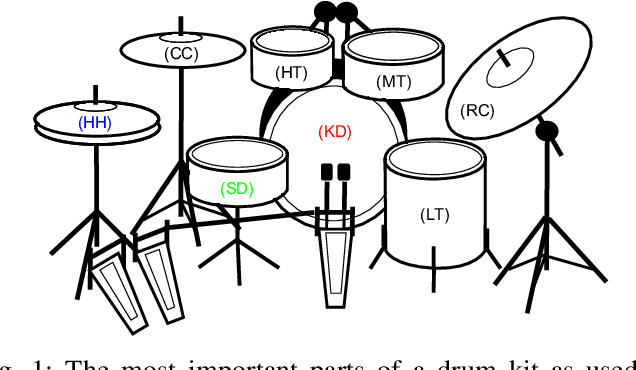
\includegraphics[scale=0.5, trim={0 1cm 0 0},clip]{figures/drumset}
    \caption{Example of the different instruments on the drumset. They are the \gls{KD}, \gls{SD}, \gls{HH}, \gls{CC}, \gls{RC}, \gls{HT}, \gls{MT}, \gls{LT}.}
    \label{DrumsetFigure}
\end{figure}

As mentioned, percussion like the drum set, stands in contrast to other musical instruments in that the different ways of playing the same instrument often differ a lot in their \textit{"audible footprint"}. The snare drum, bass drum and hi-hat all have quite different timbres, frequency span, volume, and all in all fundamentally are different instruments.

\begin{figure}[H]
    \centering
    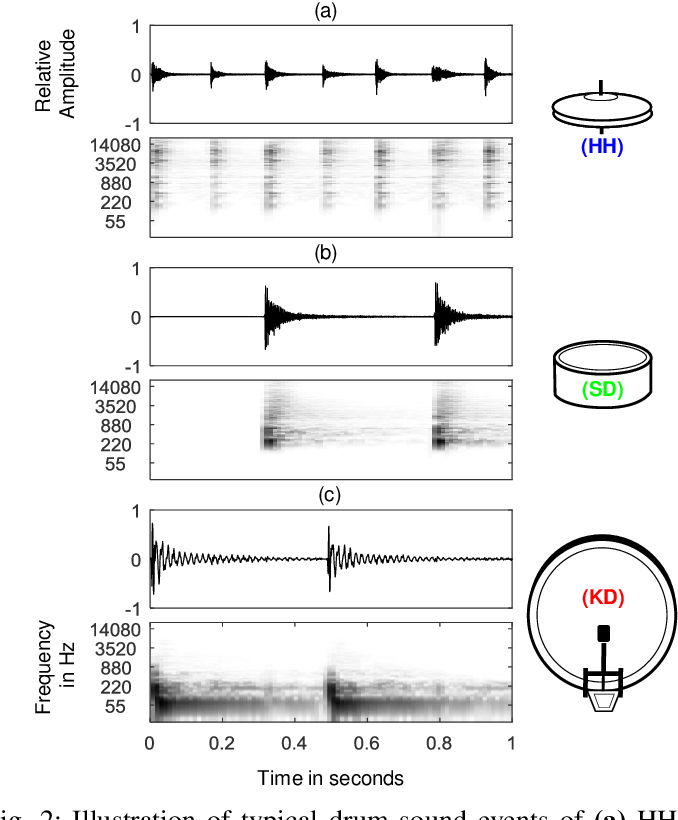
\includegraphics[scale=0.5, trim={0 1cm 0 0},clip]{figures/drumsettimbre}
    \caption{Example of the different audible footprint for drum set percussion. Plotted are the waveforms of three different drum instruments played at different speeds, together with its corresponding spectrogram. As we can see, each instrument event different significantly in how they look in and affect the spectrogram.}
    \label{DrumsetTimbreFigure}
\end{figure}

\textcolor{red}{Mention the different drum set instruments. Mention how they all have different musical properties, like frequency, timbre, etc (show waveforms maybe?). Also mention the most fundemental ones, and how Bass, snare and hi-hat are more important than e.g. the mid-tom or something.}

\section{Transcription Task}

\textcolor{red}{\textbf{An introduction to the task, with an image overview over the pipeline (Waveform $\rightarrow$ Spectrogram $\rightarrow$ Neural Network $\rightarrow$ Activation Functions $\rightarrow$ Transcription) should be done here, and is natural to give the reader a thorough understanding of the task before any other information. Understanding the task is the most important part!}}

\begin{figure}[H]
    \centering
    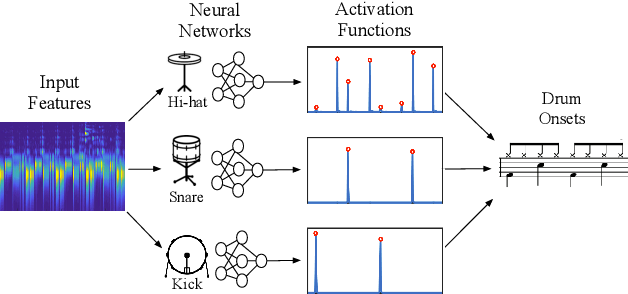
\includegraphics[scale=0.5]{figures/activations.png}
    \caption{Example of what the prediction pipeline of an \gls{ADT} model would look like, and how it transcribes instruments played in an input spectrogram.}
    \label{ADTFigure}
\end{figure}

\section{Audio}

Sound has be described as \textit{"the sensation caused in the nervous system by vibration of the delicate membranes of the ear."}~\cite{1953fundamentals}. In short, sound is the human perception of acoustic waves in a transition medium, like air. These waves, consisting of vibrating molecules, get sensed by our auditory organs and perceived by the brain. 

Thus sound can be described as the propogation and perception of waves. Mathematically, waves can be studied as signals~\cite{8454362}. To represent these sounds digitally, as \textit{audio}, one can express these waves as a signal, giving rise to the \textit{waveform}. The waveform is a representation of a signal as a graph, and charts the amplitude, or strength of the signal, over time.

\begin{figure}[H]
    \centering
    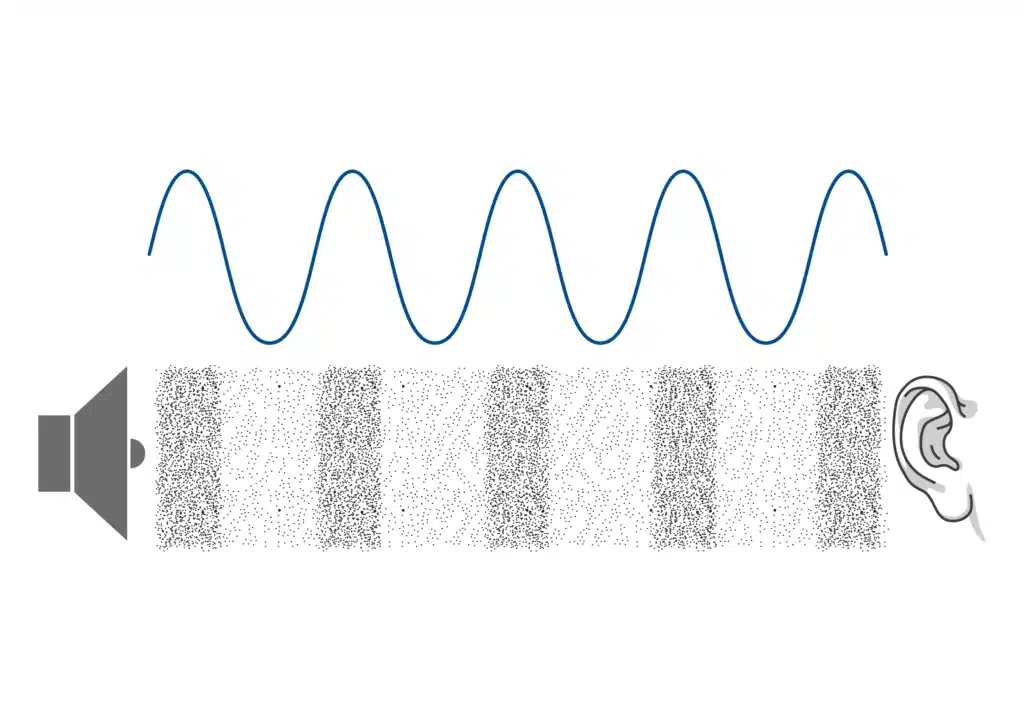
\includegraphics[scale=0.3]{figures/waveform}
    \caption{Soundwave to waveform relationship}
    \label{WaveformFigure}
\end{figure}

For monophonic sound, this waveform is a one-dimensional representation. Even though this is an excellent way of storing audio digitally, it is very compact. There have been deep learning models working directly with these waveforms, e.g. Oord et al.'s WaveNet~\cite{oord2016wavenetgenerativemodelraw}, however the task of parsing and perceiving such a signal is a complex one.

\subsection{Fourier Transform}

The Fourier Transform is a mathematical transformation which, given a frequency, computes its significance, or intensity, in a given signal. As we've established, audio is represented as a signal, and we can therefore use this transform to turn this audio signal into frequency space. 

The fourier transform is a complex transformation. Given a signal $f$, we can compute the integral \[ \widehat{f}(\xi) = \int^{\infty}_{-\infty}{f(x)e^{-i2\pi \xi x} dx} \] for a frequency $\xi$, resulting in a \textit{complex} number. This number consists of a \textit{real} part and an \textit{imaginary} part. The real part consists of the amplitude of a certain frequency, where as the imaginary part consists of the phase. This information is what allows us to, for a given signal, figure out which frequencies it is made out of and how much each frequency contributes.

By doing such a transform, we turn our temporal data into spectral data. This initively \textit{untangles} our signal into its respective base frequencies. Such an transformation could lessen the complexity of the task, making \textit{understanding} of audio easier.

\begin{figure}[H]
    \centering
    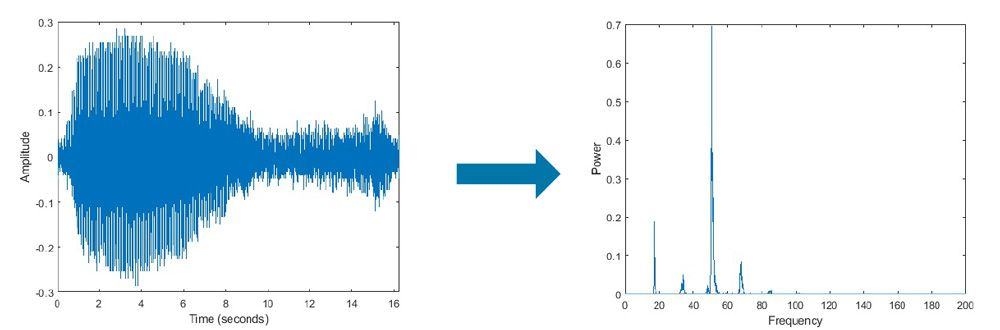
\includegraphics[scale=0.4]{figures/fft.jpg}
    \caption{Application of a Fourier Transform}
    \label{FTFigure}
\end{figure}

Note that the Fourier Transform is invertible, meaning that, given information about each frequency, we can perform a similar integral and reconstruct the original signal. In signal processing, this property is exploited heavily.

\subsection{Discrete Fourier Transform}

The Fourier Transform is defined as an integral over continuous time. On computers, instead of storing signals continuously we store signals using a discrete number of samples. Each signal's \textit{sampling rate} describes how many samples a signal contains per second of audio, and is denoted in \textit{Hz}.

To extract frequency values from these signals, we instead have to use the \gls{DFT}. Intuitively this works as the normal Fourier Transform, but ported to work on discrete-valued signals. It is given by the formula \[ X_k = \sum^{N - 1}_{n=0}{x_n \cdot e^{-i 2\pi \frac{k}{N} n}}, \] where $k$ denotes the frequency and $N$ the number of discrete samples.

\begin{figure}[H]
    \centering
    %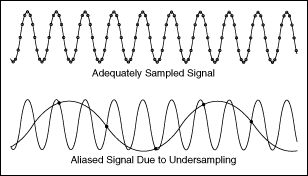
\includegraphics[scale=2.0]{figures/signalaliasing.png}
    \textcolor{red}{Add a example figure of FT vs DFT}
    %\caption{Example of aliasing in an undersampled signal.}
    %\label{AliasingFigure}
\end{figure}

\subsection{Nyquist frequency}

When we discretize a signal, e.g. when going from continuous audio waves in the air to discrete audio signals on a computer, we could lose some information. The discrete representation of the signal is an \textit{approximation} which quality is directly dependent on the sampling rate. The higher the sampling rate, the \textit{closer} we are to the original, continuous signal. However a higher sampling rate comes at the cost of needing to store these signals at a higher precision. A lower sampling rate would need less information stored, but this could also mean a less precise signal approxmation.

\textit{Aliasing} is the phenomena where new frequencies seem to emerge in undersampled signals. For a given discrete signal, the \textit{Nyquist frequency}, equal to half the sampling rate, is the maximum frequency a signal accurately can represent. Thus to prevent aliasing, one would need to store a signal with a sampling rate of at least double the maximum frequency.

\begin{figure}[H]
    \centering
    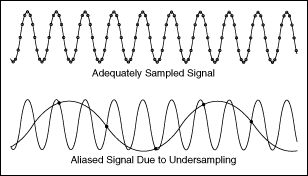
\includegraphics[scale=2.0]{figures/signalaliasing.png}
    \caption{Example of aliasing in an undersampled signal.}
    \label{AliasingFigure}
\end{figure}

Regarding the \gls{DFT}, it here directly follows that the maximum frequency we accurately could extract information about is proportional to the sampling rate of the signal.

\subsection{Fast Fourier Transform}

Keen-eyed computer scientists may have spotted that the \gls{DFT} runs in $\mathcal{O}(n^2)$ time as we, for every frequency in the range $[0, N]$ have to sum over $N$ different values. In other words, the \gls{DFT} algorithm scales quite poorly. Take into account that the standard sampling rate for audio is $44.1 \text{kHz}$, i.e. $44100 \text{Hz}$, then we can see that the \gls{DFT} could be inefficient.~\cite{pras2010sampling}

The \gls{FFT} is an algorithm which solves this problem, and instead computes the \gls{DFT} of a signal within $\mathcal{O}(n\log{n})$ time. Described by Gilbert Strang as \textit{"the most important numerical algorithm of our lifetime"}~\cite{strang1993wavelet}, this practically solves our scaling problem, and allows us to efficiently extract spectral information from a signal regardless of sampling rate.

There exist many different implementations of the \gls{FFT}. However the Cooley-Tukey algorithm is by far the most used \gls{FFT} and optimizes calculations through a \textit{divide and conquer} approach, utilizing previous calculations to compute others.~\cite{d3ea2d52-5ab2-3128-8b80-efb85267295d}

\subsection{Short-time Fourier Transform}

The Fourier Transform comes with some drawbacks, notably how by moving from time space into frequency space, we lose temporal information. For certain tasks this might be sufficient, but the temporal dimension is vital when working with transcriptions and \gls{ADT} tasks. We've seen how the Fourier Transform computes the frequencies of a signal, but what happens if we had applied the same transform to smaller, \textit{partitions} of a signal.

This leads us to the \gls{STFT}. By instead of transforming the whole signal, we transform smaller \textit{windows}, we could gain insight into the frequency space while keeping temporal information relatively intact. This turns our data from being one-dimensional into two-dimensional, giving us insight into the intensities of different frequencies, along different timesteps.

\textcolor{red}{Talk more about the partitioning. The window functions applied, and why. Spectral leakage..}

\begin{figure}[H]
    \centering
    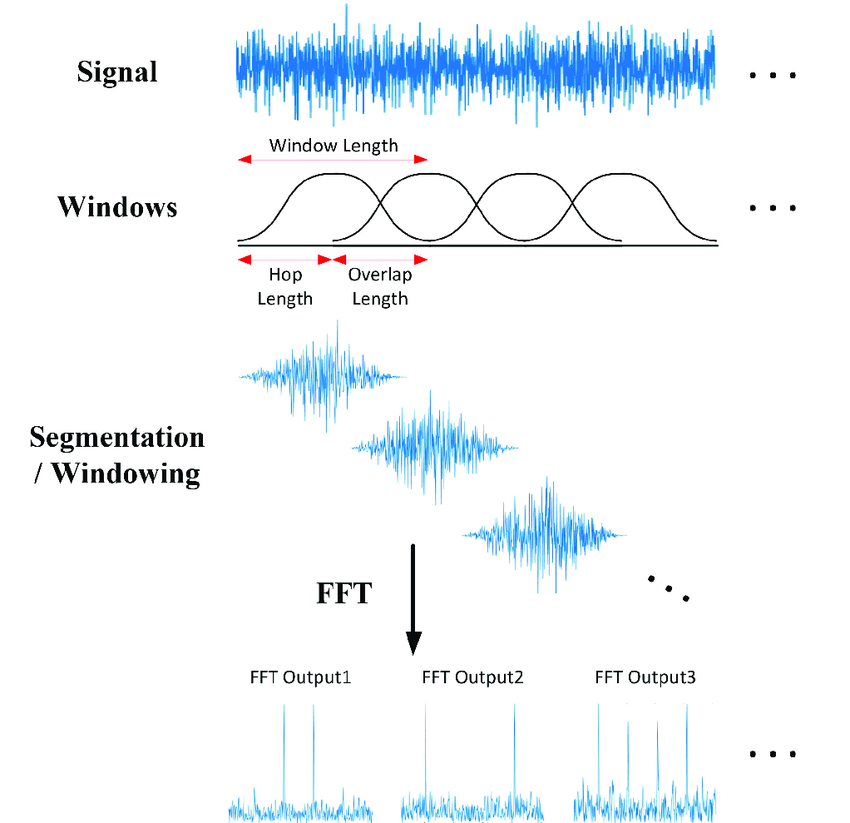
\includegraphics[scale=0.35]{figures/stft}
    \caption{Example of the \gls{STFT}}
    \label{STFTFigure}
\end{figure}

\subsection{Spectrogram}

The \gls{STFT}, as the standard Fourier Transform, returns the data as complex values. To turn these into strictly real values without discarding data, we could compute the spectrogram. This is done by squaring the absolute value of each complex number. 

This results in a 2-dimensional, real representation of our signal. A representation like this is equivalent to an \textit{image}, but can also still be modelled as a time series. In this way, we've converted our audible information into visual information. Naturally, these spectrograms can be visualized using e.g. a heatmap.

\begin{figure}[H]
    \centering
    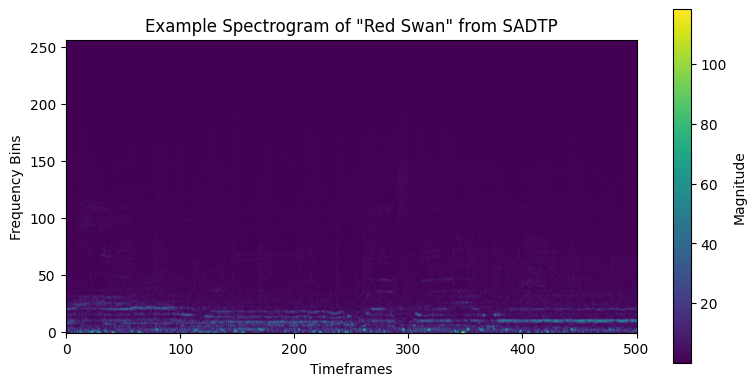
\includegraphics[scale=0.35]{figures/spectrogram}
    \caption{Heatmap of an audio spectrogram.}
    \label{SpectrogramFigure}
\end{figure}

One drawback about the spectrogram is that it contains no information about the phase of the signal it represents. That means it will not be possible to reverse the process and recreate the exact original signal. However, one could try to create an approximation like is done with the Griffin-Lim algorithm~\cite{1164317}.

\subsection{Filters}

Signal frequencies and human perception have a special relationship. We humans percieve logarithmic differences in frequencies as a linear difference in pitch, and we tend to be better at distinguishing differences in lower frequencies than higher. E.g., the notes $\text{A}_2$ and $\text{B}_2$ have the same perceptual pitch difference as $\text{D}_7$ and $\text{E}_7$, even though their difference in frequency, $\text{B}_2 - \text{A}_2 \approx 13.471 \text{Hz}$ and $\text{E}_7 - \text{D}_7 \approx 287.703 \text{Hz}$, are vastly different. As the frequency bins in a spectrogram are linearly spaced, this leads to the spectrogram not representing each frequency equally compared to our perception.

To solve this, we can filter the spectrogram into different bins, more suited to represent our perception of sound. This filtering is done by matrix multiplying our spectrogram with a \textit{filterbank}; a matrix representation of different filters.

\subsubsection{Mel Spectrograms}

The mel scale, presented by Stevens, Volkmann, and Newmann in 1937, is a transformation from the frequency scale to the mel scale. These mels have the property such that a linear difference in mels are percieved as linear differences in pitch. Application of mel-filters result in the \textit{mel spectrogram}, and are widely used when dealing with audio in machine learning, and successful applications have been seen in \gls{AMT}.~\cite{wolfmonheim2024spectralrhythmfeaturesaudio, gardner2022mt3multitaskmultitrackmusic, chang2024yourmt3+, 8350302, gong2021astaudiospectrogramtransformer, zehren2024analyzingreducingsynthetictorealtransfer}

\subsubsection{Logarithmic Filters}

The mel scale was created to mimic human perception of sound, however within \gls{ADT} there is a different trend. By instead using logarithmically spaced filters, centered on the note $\text{A}_4$, we get a \textit{logarithmically filtered spectrogram}. Intuitively one could assume this, instead of mimicing human perception, ports the spectrogram into a format preserving musical relationship and information. This seems to be a standard for \gls{ADT} and has been used extensively by the likes of Vogl et al.~\cite{8350302, vogl2018multiinstrumentdrumtranscription, Vogl2017DrumTV, signals4040042}

\begin{figure}[H]
    \centering
    %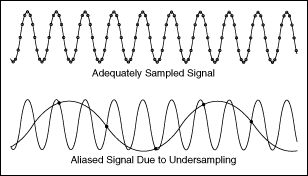
\includegraphics[scale=2.0]{figures/signalaliasing.png}
    \textcolor{red}{Add a example figure of Spectrogram vs Mel vs Logarithmic}
    %\caption{Example of aliasing in an undersampled signal.}
    %\label{AliasingFigure}
\end{figure}

\section{Transcription}

Transcription refers to a process in which we convert information from an audible format, like music, to another medium. This medium then contains a \textit{description} of said audio. As we focus on a musical context, there are a few notable such mediums.

\subsection{Sheet Music}

Sheet music is a written transcription using musical notation that, for a given instrument, contains the \textit{recipe} for a musician to play parts of the original recording. This is the standard when it comes to printing arrangements, and is extensively used by musicians.

Sheet music is typically descriptively exhaustive, and could contain information about musical properties like instrument onsets, tempo, velocity, etc. 

\begin{figure}[H]
    \centering
    
\includegraphics[scale=1.0]{figures/drumsheet}
    \caption{Example sheet music for a drumset}
    \label{DrumsheetFigure}
\end{figure}

\subsection{MIDI Annotations}

\gls{MIDI} is the industry standard for handling music digitally. It is a binary format, containing sequences of commands that allow digital interfaces to \textit{synthesize} music. As it is binary, it is unreadable to us humans without translating it into another format. When computers play \gls{MIDI} arrangements, the \gls{MIDI} sequences are parsed at a constant speed, playing different sounds through \textit{note on}/\textit{note off} events, delayed by time \textit{deltas}. Similar to sheet music, \gls{MIDI} is also very descriptive. And one could say that, intuitively, \gls{MIDI} is to a computer what sheet music is to a musician.

Recently, outputting transcriptions in a \gls{MIDI}-like format has been attempted in \gls{DTM}, and has shown to be promising. Utilizing a sequence-to-sequence \gls{NLP} approach, Gardner et al. presented MT3~\cite{gardner2022mt3multitaskmultitrackmusic}, a model inputting spectrograms and outputting \gls{MIDI} events autoregressively. This format was expanded on by Chang et al.'s YourMT3+~\cite{chang2024yourmt3+}, using a \gls{LLM} instead.

\begin{figure}[H]
    \centering
    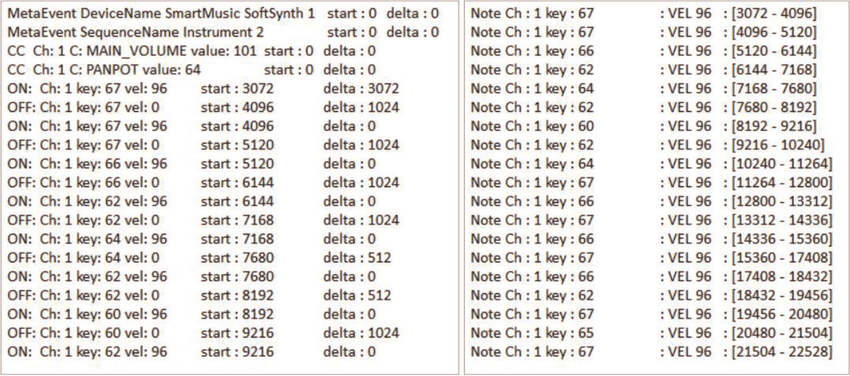
\includegraphics[scale=0.5, trim={0 0 13.8cm 0},clip]{figures/midi}
    \caption{Example MIDI arrangement in a readable format}
    \label{MIDIFigure}
\end{figure}

\subsection{Activation Functions}

In machine learning, the task of detecting instrument onsets could be described as a multi-label sequence labeling task. This involves, for each timeframe in a sequence, predicting a probability, or rather confidence value, that a certain instrument onset happens. In the domain of \gls{MIR} and \gls{AMT}, it has become common place to describe these confidence distributions as \textit{activation functions}; not to be confused with the general deep learning term, activation functions like ReLU or sigmoid.~\cite{Southall2016AutomaticDT, vogl2018multiinstrumentdrumtranscription}

This way of frame-level prediction is extensively used within onset detection in \gls{ADT} and is the approach we will be taking in this thesis.

\begin{figure}[H]
    \centering
    %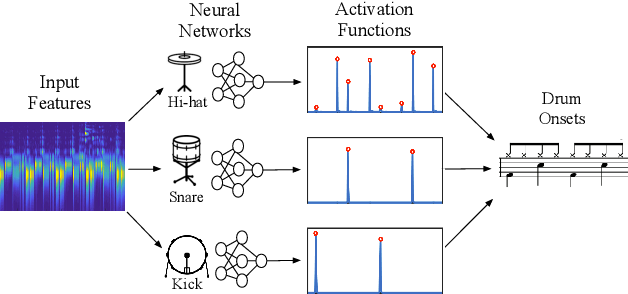
\includegraphics[scale=0.5]{figures/activations.png}
    \textcolor{red}{Need an isolated example of activation functions and respective labels.}
    \caption{Example of \gls{ADT} activation function output}
    \label{ActivationsFigure}
\end{figure}

\subsubsection{Peak-picking}

When predicting activation functions, we need a separate post-processing step to turn these confidence distributions into onset events. By utilizing a standard \textit{peak-picking} algorithm, we can isolate and enhance peaks in these activation functions, and go from a continuous distribution to a collection of discrete events.

The peak-picking algorithm, introduced in its current form by Böck et al.~\cite{Bck2012EvaluatingTO}, defines that a prediction $\hat{y}_n$ at timeframe $n$ is a \textit{peak} if it fulfills the three conditions:
\begin{align*} 
    \hat{y}_n &= \text{max}(\hat{y}_{n - m}, ..., \hat{y}_n, ... \hat{y}_{n + m}), \\ 
    \hat{y}_n &\ge \text{mean}(\hat{y}_{n - a}, ..., \hat{y}_n, ... \hat{y}_{n + a}) + \delta, \\
    n &\ge n_\text{last onset} + w.
\end{align*}

For appropriately trained deep learning models, Vogl et al.~\cite{vogl2018multiinstrumentdrumtranscription} showed that the peak-picking parameters which gave the best results were $m = a = w = 2$ and $\delta = 0.1$.

\section{Performance Measure}

\subsection{Correct Predictions}

Our machine learning models predict instrument onset events on a frame-level basis. In other words, are predictions are very granular, and we need some way to decide when a prediction is correct versus incorrect. In \gls{ADT}, a standard has become to allow a \textit{tolerance window} where event predictions are correct if they lie within a certain time window, often between $25\text{ms}$ and $50\text{ms}$. A side effect of this is that, by shifting our focus to predicted events, we lose information about \textit{not} predicting any events~\cite{vogl2016recurrent}.

\subsection{Accuracy}

For classification tasks, a standard performance measure would be \textit{accuracy}: \[ \text{Accuracy} = \frac{\text{TP} + \text{TN}}{\text{TP} + \text{TN} + \text{FP} + \text{FN}}.\] Summing up correct predictions, \gls{TP} and \gls{TN}, and dividing by total number of predictions, sum of \gls{TP}, \gls{TN}, \gls{FP} and \gls{FN}, we find a model's probability of having a correct prediction.

This performance measure falls short in that it is very susceptible to imbalanced datasets. In \gls{ADT}, most timeframes contain no onset, meaning a naïve predictor would get a high accuracy by never predicting any onsets. Another problem with accuracy is that, due to our tolerance window approach we do not have quantities for \gls{TN}, such that the standard accuracy computation is incomputable.

\subsection{F1-score}

Mentioned above are some of the reasons why \textit{F1-score} has become the typical performance measure within \gls{ADT}. F1-score combines and tries to maximize two different performance measures, namely \textit{precision}; \[ \text{Precision} = \frac{\text{TP}}{\text{TP} + \text{FP}}, \] and \textit{recall}; \[ \text{Recall} = \frac{\text{TP}}{\text{TP} + \text{FN}}. \]

The precision of a model can tell us how good it is at \textit{hitting} predictions. \textit{Perfect precision} happens when a model has no \gls{FP}, i.e. never predicting an event where one doesn't happen. Recall is similar, but represents the other end of the stick. It tells us how good a model is at \textit{not missing} predictions. \textit{Perfect recall} happens when a model has no \gls{FN}, i.e. never \textit{not} predicting an event where one does happen.

As mentioned, F1-score combines these two measures in an aggregate performance measure by computing their harmonic mean: $$ \text{F1-score} = \frac{2 \cdot \text{Precision} \cdot \text{Recall}}{\text{Precision} + \text{Recall}}. $$ By maximizing F1, we simultaneously maximize both precision and recall as well, reaping all their benefits.

\subsection{Micro vs. Macro}

There are different ways of computing and combining F1-score on multi-label data. Even though they might seem similar, they fundamentally represent different information, and thus the choice in which one to select is crucial.

\textit{Macro F1-score} is computed through the arithmetic mean of the classwise computed F1-scores. Finding a model which maximizes this measure would be similar to finding the model which performes best on each of the separate classes, preventing a class from taking priority due to imbalanced datasets. Relating this to \gls{ADT}, it would mean focusing on transcribing each instrument equally well.

\textit{Micro F1-score} is computed through finding the F1-score with global \gls{TP}, \gls{FP}, \gls{FN} values. Maximizing this would mean prioritizing classes that occur more frequently in the datasets. Such as in \gls{ADT}, this would mean focusing on transcribing instruments which appear often, like the snare or base drum, over rarer instruments like the toms.

For \gls{ADT}, the trend has been to select Micro F1-score as the main performance measure, due to its ability to show a model's \textit{general} performance on musical pieces. We want our model to maximize their ability to transcribe music, not maximize their ability to transcribe each instrument in said music. \gls{ADT}, prioritizing frequent instruments is relevant. As mentioned previously, the more frequent instruments lay the ground work for the fundamentals, and could be said to be more important than scarcely occuring ones.

\chapter{Architectures}\label{Architectures}

Finding a suitable architecture is a vital step in creating a well-performant deep learning model. By leveraging different techniques, we balance introduction of inductive biases and possibility for complexity, which hopefully can help us end up with a generalizing model.

\section{Recurrent Neural Network}

The \gls{RNN} is a standard architecture when it comes prediction on sequence data. It has been tried and tested, showing promising results for audio tasks.

The fundamental building block for \gls{RNN}s is the \textit{recurrent unit}. It iterates the whole input sequence, storing information from previous timesteps in a form of memory, through maintenance of a \textit{hidden state}. This can be extended to gaining information about future timesteps by using \textit{bidirectional} versions. In this way, prediction on current timesteps are affected by the information from surrounding timesteps. This is relevant in tasks such as \gls{ADT} as auditory information usually spreads over several timesteps, e.g. the timbre of an instrument event lingering after onset.

\begin{figure}[H]
    \centering
    \usetikzlibrary{positioning, chains, shapes.geometric, fit, shapes, arrows.meta, calc, backgrounds}

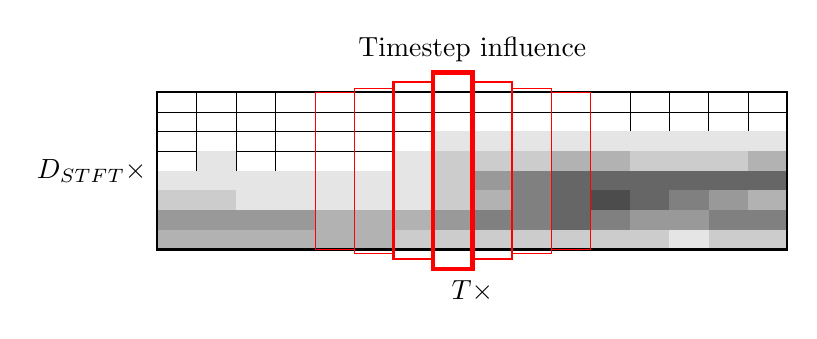
\begin{tikzpicture}[
    very thick,
    arrow/.style={
        -latex,
        very thick,
        rounded corners=0.2cm
    },
    ]

% ------ Grid ------

\draw[transform canvas={xscale=2}, step=0.25cm, ultra thin] (-2, 1) grid (2, 3);
\node[anchor=south] at (0, 3.25) {Timestep influence};
\node[anchor=east] at (-4, 2) {$D_\text{STFT}\times$};
\node[anchor=north] at (0, 0.75) {$T\times$};

% ------ Values ------

\fill[black!30] (-4.0, 1.0) rectangle (-3.5, 1.25);
\fill[black!30] (-3.5, 1.0) rectangle (-3.0, 1.25);
\fill[black!30] (-3.0, 1.0) rectangle (-2.5, 1.25);
\fill[black!30] (-2.5, 1.0) rectangle (-2.0, 1.25);
\fill[black!30] (-2.0, 1.0) rectangle (-1.5, 1.25);
\fill[black!30] (-1.5, 1.0) rectangle (-1.0, 1.25);
\fill[black!20] (-1.0, 1.0) rectangle (-0.5, 1.25);
\fill[black!20] (-0.5, 1.0) rectangle (0.0, 1.25);
\fill[black!20] (0.0, 1.0) rectangle (0.5, 1.25);
\fill[black!20] (0.5, 1.0) rectangle (1.0, 1.25);
\fill[black!20] (1.0, 1.0) rectangle (1.5, 1.25);
\fill[black!20] (1.5, 1.0) rectangle (2.0, 1.25);
\fill[black!20] (2.0, 1.0) rectangle (2.5, 1.25);
\fill[black!10] (2.5, 1.0) rectangle (3.0, 1.25);
\fill[black!20] (3.0, 1.0) rectangle (3.5, 1.25);
\fill[black!20] (3.5, 1.0) rectangle (4.0, 1.25);
\fill[black!40] (-4.0, 1.25) rectangle (-3.5, 1.5);
\fill[black!40] (-3.5, 1.25) rectangle (-3.0, 1.5);
\fill[black!40] (-3.0, 1.25) rectangle (-2.5, 1.5);
\fill[black!40] (-2.5, 1.25) rectangle (-2.0, 1.5);
\fill[black!30] (-2.0, 1.25) rectangle (-1.5, 1.5);
\fill[black!30] (-1.5, 1.25) rectangle (-1.0, 1.5);
\fill[black!30] (-1.0, 1.25) rectangle (-0.5, 1.5);
\fill[black!40] (-0.5, 1.25) rectangle (0.0, 1.5);
\fill[black!50] (0.0, 1.25) rectangle (0.5, 1.5);
\fill[black!50] (0.5, 1.25) rectangle (1.0, 1.5);
\fill[black!60] (1.0, 1.25) rectangle (1.5, 1.5);
\fill[black!50] (1.5, 1.25) rectangle (2.0, 1.5);
\fill[black!40] (2.0, 1.25) rectangle (2.5, 1.5);
\fill[black!40] (2.5, 1.25) rectangle (3.0, 1.5);
\fill[black!50] (3.0, 1.25) rectangle (3.5, 1.5);
\fill[black!50] (3.5, 1.25) rectangle (4.0, 1.5);
\fill[black!20] (-4.0, 1.5) rectangle (-3.5, 1.75);
\fill[black!20] (-3.5, 1.5) rectangle (-3.0, 1.75);
\fill[black!10] (-3.0, 1.5) rectangle (-2.5, 1.75);
\fill[black!10] (-2.5, 1.5) rectangle (-2.0, 1.75);
\fill[black!10] (-2.0, 1.5) rectangle (-1.5, 1.75);
\fill[black!10] (-1.5, 1.5) rectangle (-1.0, 1.75);
\fill[black!10] (-1.0, 1.5) rectangle (-0.5, 1.75);
\fill[black!20] (-0.5, 1.5) rectangle (0.0, 1.75);
\fill[black!30] (0.0, 1.5) rectangle (0.5, 1.75);
\fill[black!50] (0.5, 1.5) rectangle (1.0, 1.75);
\fill[black!60] (1.0, 1.5) rectangle (1.5, 1.75);
\fill[black!70] (1.5, 1.5) rectangle (2.0, 1.75);
\fill[black!60] (2.0, 1.5) rectangle (2.5, 1.75);
\fill[black!50] (2.5, 1.5) rectangle (3.0, 1.75);
\fill[black!40] (3.0, 1.5) rectangle (3.5, 1.75);
\fill[black!30] (3.5, 1.5) rectangle (4.0, 1.75);
\fill[black!10] (-4.0, 1.75) rectangle (-3.5, 2.0);
\fill[black!10] (-3.5, 1.75) rectangle (-3.0, 2.0);
\fill[black!10] (-3.0, 1.75) rectangle (-2.5, 2.0);
\fill[black!10] (-2.5, 1.75) rectangle (-2.0, 2.0);
\fill[black!10] (-2.0, 1.75) rectangle (-1.5, 2.0);
\fill[black!10] (-1.5, 1.75) rectangle (-1.0, 2.0);
\fill[black!10] (-1.0, 1.75) rectangle (-0.5, 2.0);
\fill[black!20] (-0.5, 1.75) rectangle (0.0, 2.0);
\fill[black!40] (0.0, 1.75) rectangle (0.5, 2.0);
\fill[black!50] (0.5, 1.75) rectangle (1.0, 2.0);
\fill[black!60] (1.0, 1.75) rectangle (1.5, 2.0);
\fill[black!60] (1.5, 1.75) rectangle (2.0, 2.0);
\fill[black!60] (2.0, 1.75) rectangle (2.5, 2.0);
\fill[black!60] (2.5, 1.75) rectangle (3.0, 2.0);
\fill[black!60] (3.0, 1.75) rectangle (3.5, 2.0);
\fill[black!60] (3.5, 1.75) rectangle (4.0, 2.0);
\fill[black!10] (-3.5, 2.0) rectangle (-3.0, 2.25);
\fill[black!10] (-1.0, 2.0) rectangle (-0.5, 2.25);
\fill[black!20] (-0.5, 2.0) rectangle (0.0, 2.25);
\fill[black!20] (0.0, 2.0) rectangle (0.5, 2.25);
\fill[black!20] (0.5, 2.0) rectangle (1.0, 2.25);
\fill[black!30] (1.0, 2.0) rectangle (1.5, 2.25);
\fill[black!30] (1.5, 2.0) rectangle (2.0, 2.25);
\fill[black!20] (2.0, 2.0) rectangle (2.5, 2.25);
\fill[black!20] (2.5, 2.0) rectangle (3.0, 2.25);
\fill[black!20] (3.0, 2.0) rectangle (3.5, 2.25);
\fill[black!30] (3.5, 2.0) rectangle (4.0, 2.25);
\fill[black!10] (-0.5, 2.25) rectangle (0.0, 2.5);
\fill[black!10] (0.0, 2.25) rectangle (0.5, 2.5);
\fill[black!10] (0.5, 2.25) rectangle (1.0, 2.5);
\fill[black!10] (1.0, 2.25) rectangle (1.5, 2.5);
\fill[black!10] (1.5, 2.25) rectangle (2.0, 2.5);
\fill[black!10] (2.0, 2.25) rectangle (2.5, 2.5);
\fill[black!10] (2.5, 2.25) rectangle (3.0, 2.5);
\fill[black!10] (3.0, 2.25) rectangle (3.5, 2.5);
\fill[black!10] (3.5, 2.25) rectangle (4.0, 2.5);

% ------ Outline ------
\draw[thick] (-4, 1) -- (4, 1) -- (4, 3) -- (-4, 3) -- cycle;

% ------ Influence ------

\draw[ultra thick, color=red] (-0.5, 0.75) -- (0, 0.75) -- (0, 3.25) -- (-0.5, 3.25) -- cycle;

\draw[thick, color=red] (-1, 0.875) -- (-0.5, 0.875) -- (-0.5, 3.125) -- (-1, 3.125) -- cycle;
\draw[thick, color=red] (0, 0.875) -- (0.5, 0.875) -- (0.5, 3.125) -- (0, 3.125) -- cycle;

\draw[thin, color=red] (-1.5, 0.95) -- (-1, 0.95) -- (-1, 3.05) -- (-1.5, 3.05) -- cycle;
\draw[thin, color=red] (0.5, 0.95) -- (1, 0.95) -- (1, 3.05) -- (0.5, 3.05) -- cycle;

\draw[ultra thin, color=red] (-2, 1) -- (-1.5, 1) -- (-1.5, 3) -- (-2, 3) -- cycle;
\draw[ultra thin, color=red] (1, 1) -- (1.5, 1) -- (1.5, 3) -- (1, 3) -- cycle;

\end{tikzpicture}
    \caption{Visualization of adjacent timestep's influence for a bidirectional RNN.}
    \label{RNNInfluenceFigure}
\end{figure}

However, traditional \gls{RNN}s suffer from the \textit{vanishing gradient problem} due to a timestep's influence diminishing with distance, making \textit{long range dependencies} harder to learn. Different architectures have been developed to try to overcome these issues, such as the \gls{GRU} by Cho et al.~\cite{DBLP:conf/emnlp/ChoMGBBSB14}, and \gls{LSTM} by Hochreiter and Schmidhuber~\cite{10.1162/neco.1997.9.8.1735}.

It has been shown that \gls{GRU}s and \gls{LSTM}s are capable of learning \gls{ADT} related tasks, and is therefore in interest to comparatively measure how their efficiency stands in regards to other architectures~\cite{Southall2016AutomaticDT, vogl2016recurrent, Vogl2017DrumTV, signals4040042}.

\subsection{Implementation}

Our \gls{RNN} architecture consists of several bidirectional recurrent units, ending in a framewise linear layer. For the \gls{BiRU}, we train both a \gls{GRU} and an \gls{LSTM} model as hyperparameters, in addition to search over number of layers $L \in \{2, 3, 4, 5, 6\}$ and hidden size $H \in \{72, 144, 288\}$, selecting the one with best performance. At last, we have a linear layer, outputting onset probabilities for each of the drums per timeframe.

\begin{figure}[H]
    \centering
    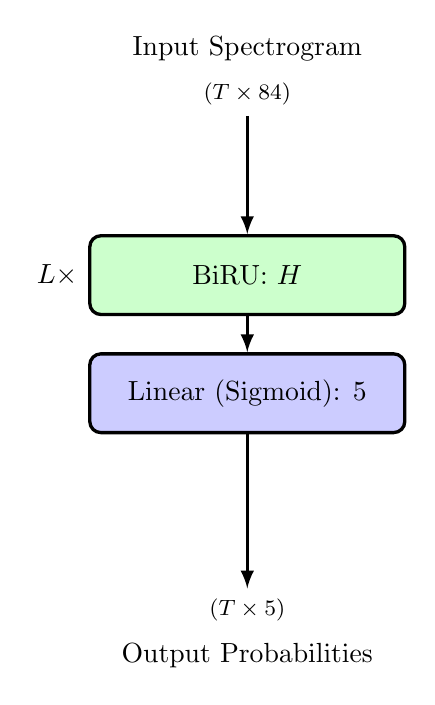
\begin{tikzpicture}[
    very thick,
    arrow/.style={
        -latex,
        very thick,
        rounded corners=0.2cm
    },
    ]

\node[anchor=south, label=above:{Input Spectrogram}] at (0, 0){\footnotesize{($T \times 84$)}};

\draw[arrow] (0, 0) -- (0, -1.5) node[rectangle, 
rounded corners, 
draw, 
anchor=north, 
label=west:$L\times$,
fill=green!20,
minimum height=1cm,
minimum width=4cm
] (a) {\acrshort{BiRU}: $H$};

\draw[arrow] (a) -- (0, -3) node[rectangle, 
rounded corners, 
draw, 
anchor=north, 
fill=blue!20,
minimum height=1cm,
minimum width=4cm
] (b) {Linear (Sigmoid): $5$};

\draw[arrow] (b) -- (0, -6);

\node[anchor=north, label=below:{Output Probabilities}] at (0, -6){\footnotesize{($T \times 5$)}};

\end{tikzpicture}
    \caption{RNN architecture structure.}
    \label{RNNFigure}
\end{figure}

\section{Convolutional Neural Network}

We've mentioned that spectrograms can be treated as images. Therefore it would make sense to try an image focused approach, by utilizing \textit{convolutions}. By applying convolutional layers, each timestep gets access to information around itself, a \textit{context}. These convolutional layers make up the primary building blocks for the \gls{CNN}.

\begin{figure}[H]
    \centering
    \begin{tikzpicture}[
    very thick,
    arrow/.style={
        -latex,
        very thick,
        rounded corners=0.2cm
    },
    ]

% ------ Grid ------

\draw[transform canvas={xscale=2}, step=0.25cm, ultra thin] (-2, 1) grid (2, 3);
\node[anchor=south] at (0, 3.25) {Contextual influence};
\node[anchor=east] at (-4, 2) {$D_\text{STFT}\times$};
\node[anchor=north] at (0, 0.75) {$T\times$};

% ------ Values ------

\fill[black!30] (-4.0, 1.0) rectangle (-3.5, 1.25);
\fill[black!30] (-3.5, 1.0) rectangle (-3.0, 1.25);
\fill[black!30] (-3.0, 1.0) rectangle (-2.5, 1.25);
\fill[black!30] (-2.5, 1.0) rectangle (-2.0, 1.25);
\fill[black!30] (-2.0, 1.0) rectangle (-1.5, 1.25);
\fill[black!30] (-1.5, 1.0) rectangle (-1.0, 1.25);
\fill[black!20] (-1.0, 1.0) rectangle (-0.5, 1.25);
\fill[black!20] (-0.5, 1.0) rectangle (0.0, 1.25);
\fill[black!20] (0.0, 1.0) rectangle (0.5, 1.25);
\fill[black!20] (0.5, 1.0) rectangle (1.0, 1.25);
\fill[black!20] (1.0, 1.0) rectangle (1.5, 1.25);
\fill[black!20] (1.5, 1.0) rectangle (2.0, 1.25);
\fill[black!20] (2.0, 1.0) rectangle (2.5, 1.25);
\fill[black!10] (2.5, 1.0) rectangle (3.0, 1.25);
\fill[black!20] (3.0, 1.0) rectangle (3.5, 1.25);
\fill[black!20] (3.5, 1.0) rectangle (4.0, 1.25);
\fill[black!40] (-4.0, 1.25) rectangle (-3.5, 1.5);
\fill[black!40] (-3.5, 1.25) rectangle (-3.0, 1.5);
\fill[black!40] (-3.0, 1.25) rectangle (-2.5, 1.5);
\fill[black!40] (-2.5, 1.25) rectangle (-2.0, 1.5);
\fill[black!30] (-2.0, 1.25) rectangle (-1.5, 1.5);
\fill[black!30] (-1.5, 1.25) rectangle (-1.0, 1.5);
\fill[black!30] (-1.0, 1.25) rectangle (-0.5, 1.5);
\fill[black!40] (-0.5, 1.25) rectangle (0.0, 1.5);
\fill[black!50] (0.0, 1.25) rectangle (0.5, 1.5);
\fill[black!50] (0.5, 1.25) rectangle (1.0, 1.5);
\fill[black!60] (1.0, 1.25) rectangle (1.5, 1.5);
\fill[black!50] (1.5, 1.25) rectangle (2.0, 1.5);
\fill[black!40] (2.0, 1.25) rectangle (2.5, 1.5);
\fill[black!40] (2.5, 1.25) rectangle (3.0, 1.5);
\fill[black!50] (3.0, 1.25) rectangle (3.5, 1.5);
\fill[black!50] (3.5, 1.25) rectangle (4.0, 1.5);
\fill[black!20] (-4.0, 1.5) rectangle (-3.5, 1.75);
\fill[black!20] (-3.5, 1.5) rectangle (-3.0, 1.75);
\fill[black!10] (-3.0, 1.5) rectangle (-2.5, 1.75);
\fill[black!10] (-2.5, 1.5) rectangle (-2.0, 1.75);
\fill[black!10] (-2.0, 1.5) rectangle (-1.5, 1.75);
\fill[black!10] (-1.5, 1.5) rectangle (-1.0, 1.75);
\fill[black!10] (-1.0, 1.5) rectangle (-0.5, 1.75);
\fill[black!20] (-0.5, 1.5) rectangle (0.0, 1.75);
\fill[black!30] (0.0, 1.5) rectangle (0.5, 1.75);
\fill[black!50] (0.5, 1.5) rectangle (1.0, 1.75);
\fill[black!60] (1.0, 1.5) rectangle (1.5, 1.75);
\fill[black!70] (1.5, 1.5) rectangle (2.0, 1.75);
\fill[black!60] (2.0, 1.5) rectangle (2.5, 1.75);
\fill[black!50] (2.5, 1.5) rectangle (3.0, 1.75);
\fill[black!40] (3.0, 1.5) rectangle (3.5, 1.75);
\fill[black!30] (3.5, 1.5) rectangle (4.0, 1.75);
\fill[black!10] (-4.0, 1.75) rectangle (-3.5, 2.0);
\fill[black!10] (-3.5, 1.75) rectangle (-3.0, 2.0);
\fill[black!10] (-3.0, 1.75) rectangle (-2.5, 2.0);
\fill[black!10] (-2.5, 1.75) rectangle (-2.0, 2.0);
\fill[black!10] (-2.0, 1.75) rectangle (-1.5, 2.0);
\fill[black!10] (-1.5, 1.75) rectangle (-1.0, 2.0);
\fill[black!10] (-1.0, 1.75) rectangle (-0.5, 2.0);
\fill[black!20] (-0.5, 1.75) rectangle (0.0, 2.0);
\fill[black!40] (0.0, 1.75) rectangle (0.5, 2.0);
\fill[black!50] (0.5, 1.75) rectangle (1.0, 2.0);
\fill[black!60] (1.0, 1.75) rectangle (1.5, 2.0);
\fill[black!60] (1.5, 1.75) rectangle (2.0, 2.0);
\fill[black!60] (2.0, 1.75) rectangle (2.5, 2.0);
\fill[black!60] (2.5, 1.75) rectangle (3.0, 2.0);
\fill[black!60] (3.0, 1.75) rectangle (3.5, 2.0);
\fill[black!60] (3.5, 1.75) rectangle (4.0, 2.0);
\fill[black!10] (-3.5, 2.0) rectangle (-3.0, 2.25);
\fill[black!10] (-1.0, 2.0) rectangle (-0.5, 2.25);
\fill[black!20] (-0.5, 2.0) rectangle (0.0, 2.25);
\fill[black!20] (0.0, 2.0) rectangle (0.5, 2.25);
\fill[black!20] (0.5, 2.0) rectangle (1.0, 2.25);
\fill[black!30] (1.0, 2.0) rectangle (1.5, 2.25);
\fill[black!30] (1.5, 2.0) rectangle (2.0, 2.25);
\fill[black!20] (2.0, 2.0) rectangle (2.5, 2.25);
\fill[black!20] (2.5, 2.0) rectangle (3.0, 2.25);
\fill[black!20] (3.0, 2.0) rectangle (3.5, 2.25);
\fill[black!30] (3.5, 2.0) rectangle (4.0, 2.25);
\fill[black!10] (-0.5, 2.25) rectangle (0.0, 2.5);
\fill[black!10] (0.0, 2.25) rectangle (0.5, 2.5);
\fill[black!10] (0.5, 2.25) rectangle (1.0, 2.5);
\fill[black!10] (1.0, 2.25) rectangle (1.5, 2.5);
\fill[black!10] (1.5, 2.25) rectangle (2.0, 2.5);
\fill[black!10] (2.0, 2.25) rectangle (2.5, 2.5);
\fill[black!10] (2.5, 2.25) rectangle (3.0, 2.5);
\fill[black!10] (3.0, 2.25) rectangle (3.5, 2.5);
\fill[black!10] (3.5, 2.25) rectangle (4.0, 2.5);

% ------ Outline ------
\draw[thick] (-4, 1) -- (4, 1) -- (4, 3) -- (-4, 3) -- cycle;

% ------ Influence ------

\draw[ultra thick, color=red, pattern=north east lines, pattern color=red] (-0.5, 1) -- (0, 1) -- (0, 3) -- (-0.5, 3) -- cycle;

\draw[thick, color=red] (-1, 1) -- (0.5, 1) -- (0.5, 3.) -- (-1, 3) -- cycle;


\end{tikzpicture}
    \caption{Visualization of a timestep's contextual influence with CNNs.}
    \label{CNNInfluenceFigure}
\end{figure}

\gls{CNN}s have been shown to give reasonable performance within \gls{ADT}. This could be due to contextual information being important for identifying instrument onsets, and making learning easier for our models~\cite{Vogl2017DrumTV}.

\subsection{Implementation}

Our \gls{CNN} architecure consists of $I \in \{1, 2, 3\}$ initial convolutional blocks. Inside this block, convolutional layers have an increasing number of kernels $C = \{32, 64, 96\}$, intuitively leading to an increase in complexity along with depth. Then we have a varying amount of fully connected layers $L \in \{1, 2, 3, 4\}$, projecting into a latent space sized $H \in \{72, 144, 288, 576\}$. Both the convolutional and fully connected layers are followed by a \gls{ReLU} activation function. Lastly, an output layer computed each instrument's onset probabilities.

\begin{figure}[H]
    \centering
    \begin{tikzpicture}[
    very thick,
    arrow/.style={
        -latex,
        very thick,
        rounded corners=0.2cm
    },
    ]

\node[anchor=south, label=above:{Input Spectrogram}] at (0, -0.5){\footnotesize{($T \times D_\text{STFT}$)}};

\draw[arrow] (0, -0.5) -- (0, -1.5) node [rectangle,
rounded corners,
draw,
anchor=north,
fill=magenta!20,
minimum height=1cm,
minimum width=4cm
] (a) {Convolution (ReLU): $C_i$  $3 \times 3$};

\draw (a) -- (0, -2.75) node[rectangle,
rounded corners,
draw,
anchor=north,
fill=yellow!20,
minimum height=0.75cm,
minimum width=4cm
] (b) {Batch normalization};

\draw (b) -- (0, -3.825) node[rectangle,
rounded corners,
draw,
anchor=north,
fill=yellow!20,
minimum height=0.75cm,
minimum width=4cm
] (c) {Max pooling: $1 \times 3$};

\draw (c) -- (0, -4.825) node[rectangle,
rounded corners,
draw,
anchor=north,
fill=yellow!20,
minimum height=0.75cm,
minimum width=4cm
] (d) {Dropout: $p = 0.3$};

\begin{scope}[on background layer]
    \node[rectangle,
    fill=gray!20,
    rounded corners=3mm,
    label={[name=ablabel]west:$2\times$},
    draw,
    very thick,
    fit=(a) (b)] (ab) {};
    \node[rectangle,
    fill=gray!10,
    rounded corners=5mm,
    label=west:$I\times$,
    draw,
    very thick,
    fit= (ab) (ablabel) (d)] {};
    \node[rectangle,
    fill=gray!20,
    rounded corners=3mm,
    label={[name=ablabel]west:$2\times$},
    draw,
    very thick,
    fit=(a) (b)] (ab) {};
\end{scope}


\draw[arrow] (d) -- (0, -6.25) node[rectangle, 
rounded corners, 
draw, 
anchor=north, 
label=west:$L\times$,
fill=cyan!20,
minimum height=1cm,
minimum width=4cm
] (g) {Fully connected (ReLU): $H$};

\draw[arrow] (g) -- (0, -7.75) node[rectangle, 
rounded corners, 
draw, 
anchor=north, 
fill=blue!20,
minimum height=1cm,
minimum width=4cm
] (h) {Linear (Sigmoid): $5$};

\draw[arrow] (h) -- (0, -9.75);

\node[anchor=north, label=below:{Output Probabilities}] at (0, -9.75){\footnotesize{($T \times 5$)}};

\end{tikzpicture}
    \caption{CNN architecture structure.}
    \label{CNNFigure}
\end{figure}

\section[Convolutional RNN]{Convolutional Recurrent Neural Network}

The previous features, recurrent layers and convolutions, are not mutually exclusive. Theoretically they can harmonize together, complementing eachother for easier learning. This results in the \gls{CRNN} architecture.

Intuitively, the \gls{CNN}s ability to process images like the spectrogram, together with the \gls{RNN}s ability to understand temporal sequence data should prove beneficial for \gls{ADT} tasks. And indeed, this combination of cross-timestep memory and contextual data representation has shown to be insightful~\cite{Vogl2017DrumTV, vogl2018multiinstrumentdrumtranscription, signals4040042}.

\begin{figure}[H]
    \centering
    \begin{tikzpicture}[
    very thick,
    arrow/.style={
        -latex,
        very thick,
        rounded corners=0.2cm
    },
    ]

% ------ Grid ------

\draw[transform canvas={xscale=2}, step=0.25cm, ultra thin] (-2, 1) grid (2, 3);
\node[anchor=south] at (0, 3.25) {Combinative influence};
\node[anchor=east] at (-4, 2) {$D_\text{STFT}\times$};
\node[anchor=north] at (0, 0.75) {$T\times$};

% ------ Values ------

\fill[black!30] (-4.0, 1.0) rectangle (-3.5, 1.25);
\fill[black!30] (-3.5, 1.0) rectangle (-3.0, 1.25);
\fill[black!30] (-3.0, 1.0) rectangle (-2.5, 1.25);
\fill[black!30] (-2.5, 1.0) rectangle (-2.0, 1.25);
\fill[black!30] (-2.0, 1.0) rectangle (-1.5, 1.25);
\fill[black!30] (-1.5, 1.0) rectangle (-1.0, 1.25);
\fill[black!20] (-1.0, 1.0) rectangle (-0.5, 1.25);
\fill[black!20] (-0.5, 1.0) rectangle (0.0, 1.25);
\fill[black!20] (0.0, 1.0) rectangle (0.5, 1.25);
\fill[black!20] (0.5, 1.0) rectangle (1.0, 1.25);
\fill[black!20] (1.0, 1.0) rectangle (1.5, 1.25);
\fill[black!20] (1.5, 1.0) rectangle (2.0, 1.25);
\fill[black!20] (2.0, 1.0) rectangle (2.5, 1.25);
\fill[black!10] (2.5, 1.0) rectangle (3.0, 1.25);
\fill[black!20] (3.0, 1.0) rectangle (3.5, 1.25);
\fill[black!20] (3.5, 1.0) rectangle (4.0, 1.25);
\fill[black!40] (-4.0, 1.25) rectangle (-3.5, 1.5);
\fill[black!40] (-3.5, 1.25) rectangle (-3.0, 1.5);
\fill[black!40] (-3.0, 1.25) rectangle (-2.5, 1.5);
\fill[black!40] (-2.5, 1.25) rectangle (-2.0, 1.5);
\fill[black!30] (-2.0, 1.25) rectangle (-1.5, 1.5);
\fill[black!30] (-1.5, 1.25) rectangle (-1.0, 1.5);
\fill[black!30] (-1.0, 1.25) rectangle (-0.5, 1.5);
\fill[black!40] (-0.5, 1.25) rectangle (0.0, 1.5);
\fill[black!50] (0.0, 1.25) rectangle (0.5, 1.5);
\fill[black!50] (0.5, 1.25) rectangle (1.0, 1.5);
\fill[black!60] (1.0, 1.25) rectangle (1.5, 1.5);
\fill[black!50] (1.5, 1.25) rectangle (2.0, 1.5);
\fill[black!40] (2.0, 1.25) rectangle (2.5, 1.5);
\fill[black!40] (2.5, 1.25) rectangle (3.0, 1.5);
\fill[black!50] (3.0, 1.25) rectangle (3.5, 1.5);
\fill[black!50] (3.5, 1.25) rectangle (4.0, 1.5);
\fill[black!20] (-4.0, 1.5) rectangle (-3.5, 1.75);
\fill[black!20] (-3.5, 1.5) rectangle (-3.0, 1.75);
\fill[black!10] (-3.0, 1.5) rectangle (-2.5, 1.75);
\fill[black!10] (-2.5, 1.5) rectangle (-2.0, 1.75);
\fill[black!10] (-2.0, 1.5) rectangle (-1.5, 1.75);
\fill[black!10] (-1.5, 1.5) rectangle (-1.0, 1.75);
\fill[black!10] (-1.0, 1.5) rectangle (-0.5, 1.75);
\fill[black!20] (-0.5, 1.5) rectangle (0.0, 1.75);
\fill[black!30] (0.0, 1.5) rectangle (0.5, 1.75);
\fill[black!50] (0.5, 1.5) rectangle (1.0, 1.75);
\fill[black!60] (1.0, 1.5) rectangle (1.5, 1.75);
\fill[black!70] (1.5, 1.5) rectangle (2.0, 1.75);
\fill[black!60] (2.0, 1.5) rectangle (2.5, 1.75);
\fill[black!50] (2.5, 1.5) rectangle (3.0, 1.75);
\fill[black!40] (3.0, 1.5) rectangle (3.5, 1.75);
\fill[black!30] (3.5, 1.5) rectangle (4.0, 1.75);
\fill[black!10] (-4.0, 1.75) rectangle (-3.5, 2.0);
\fill[black!10] (-3.5, 1.75) rectangle (-3.0, 2.0);
\fill[black!10] (-3.0, 1.75) rectangle (-2.5, 2.0);
\fill[black!10] (-2.5, 1.75) rectangle (-2.0, 2.0);
\fill[black!10] (-2.0, 1.75) rectangle (-1.5, 2.0);
\fill[black!10] (-1.5, 1.75) rectangle (-1.0, 2.0);
\fill[black!10] (-1.0, 1.75) rectangle (-0.5, 2.0);
\fill[black!20] (-0.5, 1.75) rectangle (0.0, 2.0);
\fill[black!40] (0.0, 1.75) rectangle (0.5, 2.0);
\fill[black!50] (0.5, 1.75) rectangle (1.0, 2.0);
\fill[black!60] (1.0, 1.75) rectangle (1.5, 2.0);
\fill[black!60] (1.5, 1.75) rectangle (2.0, 2.0);
\fill[black!60] (2.0, 1.75) rectangle (2.5, 2.0);
\fill[black!60] (2.5, 1.75) rectangle (3.0, 2.0);
\fill[black!60] (3.0, 1.75) rectangle (3.5, 2.0);
\fill[black!60] (3.5, 1.75) rectangle (4.0, 2.0);
\fill[black!10] (-3.5, 2.0) rectangle (-3.0, 2.25);
\fill[black!10] (-1.0, 2.0) rectangle (-0.5, 2.25);
\fill[black!20] (-0.5, 2.0) rectangle (0.0, 2.25);
\fill[black!20] (0.0, 2.0) rectangle (0.5, 2.25);
\fill[black!20] (0.5, 2.0) rectangle (1.0, 2.25);
\fill[black!30] (1.0, 2.0) rectangle (1.5, 2.25);
\fill[black!30] (1.5, 2.0) rectangle (2.0, 2.25);
\fill[black!20] (2.0, 2.0) rectangle (2.5, 2.25);
\fill[black!20] (2.5, 2.0) rectangle (3.0, 2.25);
\fill[black!20] (3.0, 2.0) rectangle (3.5, 2.25);
\fill[black!30] (3.5, 2.0) rectangle (4.0, 2.25);
\fill[black!10] (-0.5, 2.25) rectangle (0.0, 2.5);
\fill[black!10] (0.0, 2.25) rectangle (0.5, 2.5);
\fill[black!10] (0.5, 2.25) rectangle (1.0, 2.5);
\fill[black!10] (1.0, 2.25) rectangle (1.5, 2.5);
\fill[black!10] (1.5, 2.25) rectangle (2.0, 2.5);
\fill[black!10] (2.0, 2.25) rectangle (2.5, 2.5);
\fill[black!10] (2.5, 2.25) rectangle (3.0, 2.5);
\fill[black!10] (3.0, 2.25) rectangle (3.5, 2.5);
\fill[black!10] (3.5, 2.25) rectangle (4.0, 2.5);

% ------ Outline ------
\draw[thick] (-4, 1) -- (4, 1) -- (4, 3) -- (-4, 3) -- cycle;

% ------ Influence ------

\draw[ultra thick, color=red, pattern=north east lines, pattern color=red] (-0.5, 0.75) -- (0, 0.75) -- (0, 3.25) -- (-0.5, 3.25) -- cycle;
\draw[very thick, color=red] (-1, 0.75) -- (0.5, 0.75) -- (0.5, 3.25) -- (-1, 3.25) -- cycle;

\draw[thick, color=red, pattern=north east lines, pattern color=red] (-1, 0.875) -- (-0.5, 0.875) -- (-0.5, 3.125) -- (-1, 3.125) -- cycle;
\draw[thin, color=red] (-1.5, 0.875) -- (-1, 0.875) -- (-1, 3.125) -- (-1.5, 3.125) -- cycle;
\draw[thick, color=red, pattern=north east lines, pattern color=red] (0, 0.875) -- (0.5, 0.875) -- (0.5, 3.125) -- (0, 3.125) -- cycle;
\draw[thin, color=red] (0.5, 0.875) -- (1.0, 0.875) -- (1.0, 3.125) -- (0.5, 3.125) -- cycle;

\draw[very thin, color=red, pattern=north east lines, pattern color=red] (-1.5, 0.95) -- (-1, 0.95) -- (-1, 3.05) -- (-1.5, 3.05) -- cycle;
\draw[ultra thin, color=red] (-2, 0.95) -- (-1.5, 0.95) -- (-1.5, 3.05) -- (-2, 3.05) -- cycle;
\draw[very thin, color=red, pattern=north east lines, pattern color=red] (0.5, 0.95) -- (1, 0.95) -- (1, 3.05) -- (0.5, 3.05) -- cycle;
\draw[ultra thin, color=red] (1, 0.95) -- (1.5, 0.95) -- (1.5, 3.05) -- (1, 3.05) -- cycle;


\end{tikzpicture}
    \caption{Visualization of a timestep's contextual and cross-timestep influence with Convolutional RNNs.}
    \label{CRNNInfluenceFigure}
\end{figure}

\subsection{Implementation}

We begin with a fixed-size convolutional block with $I = 2$, as used by several \gls{ADT} authors~\cite{Vogl2017DrumTV, signals4040042}. Following the \gls{CNN} it has an increasing number of kernels $C = \{32, 64\}$. We then, similar to the \gls{RNN}, have a \gls{BiRU} layer of either a \gls{GRU} or \gls{LSTM}, with number of layers $L \in \{2, 3, 4, 5\}$ and hidden size $H \in \{72, 144, 288\}$. Output probabilities are then computed through the final linear layer.

\begin{figure}[H]
    \centering
    \begin{tikzpicture}[
    very thick,
    arrow/.style={
        -latex,
        very thick,
        rounded corners=0.2cm
    },
    ]

\node[anchor=south, label=above:{Input Spectrogram}] at (0, 0){\footnotesize{($T \times D_\text{STFT}$)}};

\draw[arrow] (0, 0) -- (0, -1.5) node [rectangle,
rounded corners,
draw,
anchor=north,
fill=magenta!20,
minimum height=1cm,
minimum width=4cm
] (a) {Convolution (ReLU): $C_i$  $3 \times 3$};

\draw (a) -- (0, -2.75) node[rectangle,
rounded corners,
draw,
anchor=north,
fill=yellow!20,
minimum height=0.75cm,
minimum width=4cm
] (b) {Batch normalization};

\draw (b) -- (0, -3.825) node[rectangle,
rounded corners,
draw,
anchor=north,
fill=yellow!20,
minimum height=0.75cm,
minimum width=4cm
] (c) {Max pooling: $1 \times 3$};

\draw (c) -- (0, -4.825) node[rectangle,
rounded corners,
draw,
anchor=north,
fill=yellow!20,
minimum height=0.75cm,
minimum width=4cm
] (d) {Dropout: $p = 0.3$};

\begin{scope}[on background layer]
    \node[rectangle,
    fill=gray!20,
    rounded corners=3mm,
    label={[name=ablabel]west:$2\times$},
    draw,
    very thick,
    fit=(a) (b)] (ab) {};
    \node[rectangle,
    fill=gray!10,
    rounded corners=5mm,
    label=west:$2\times$,
    draw,
    very thick,
    fit= (ab) (ablabel) (d)] {};
    \node[rectangle,
    fill=gray!20,
    rounded corners=3mm,
    label={[name=ablabel]west:$2\times$},
    draw,
    very thick,
    fit=(a) (b)] (ab) {};
\end{scope}

\draw[arrow] (d) -- (0, -7) node[rectangle, 
rounded corners, 
draw, 
anchor=north, 
label=west:$L\times$,
fill=green!20,
minimum height=1cm,
minimum width=4cm
] (g) {BiRU: $H$};

\draw[arrow] (g) -- (0, -8.5) node[rectangle, 
rounded corners, 
draw, 
anchor=north, 
fill=blue!20,
minimum height=1cm,
minimum width=4cm
] (h) {Linear (Sigmoid): $5$};

\draw[arrow] (h) -- (0, -11.5);

\node[anchor=north, label=below:{Output Probabilities}] at (0, -11.5){\footnotesize{($T \times 5$)}};

\end{tikzpicture}
    \caption{Convolutional RNN architecture structure.}
    \label{CRNNFigure}
\end{figure}

\section{Convolutional Transformer}

Google's "Attention Is All You Need"~\cite{NIPS2017_3f5ee243} made headway in regards to sequence prediction. It introduced the \textit{Attention} layer, making a model capable of learning to \textit{attend} to different elements in a sequence, and learning the relationship between them. Models dropping the recurrent units in favour of attention blocks are called \textit{transformers}.

As mentioned, the \gls{RNN} displays difficulty in sustaining long range dependencies through its hidden state, and information further away tends to become attenuated. The attention layer solves this by allowing each element to individually attend to each other element in the sequence separately. Intuitively, it allows each element to \textit{"intelligently"} pick and choose where it wants to look, and what elements it wants to be influenced by. This stands in contrast to the recurrent units, where each element has to learn and predict what information about itself other elements could find useful, and \textit{"remembering"} that, adding it to the hidden state.

\begin{figure}[H]
    \centering
    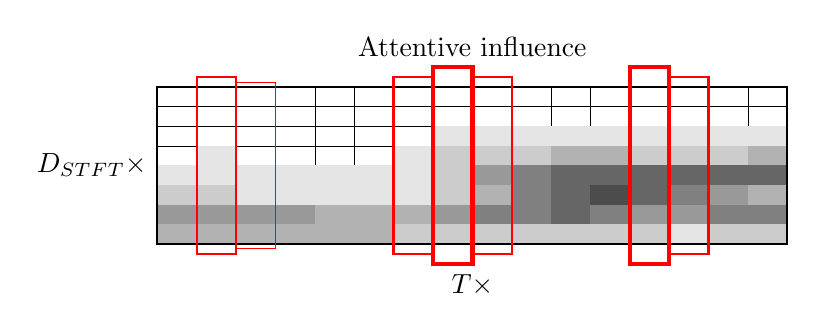
\begin{tikzpicture}[
    very thick,
    arrow/.style={
        -latex,
        very thick,
        rounded corners=0.2cm
    },
    ]

% ------ Grid ------

\draw[transform canvas={xscale=2}, step=0.25cm, ultra thin] (-2, 1) grid (2, 3);
\node[anchor=south] at (0, 3.25) {Attentive influence};
\node[anchor=east] at (-4, 2) {$D_\text{STFT}\times$};
\node[anchor=north] at (0, 0.75) {$T\times$};

% ------ Values ------

\fill[black!30] (-4.0, 1.0) rectangle (-3.5, 1.25);
\fill[black!30] (-3.5, 1.0) rectangle (-3.0, 1.25);
\fill[black!30] (-3.0, 1.0) rectangle (-2.5, 1.25);
\fill[black!30] (-2.5, 1.0) rectangle (-2.0, 1.25);
\fill[black!30] (-2.0, 1.0) rectangle (-1.5, 1.25);
\fill[black!30] (-1.5, 1.0) rectangle (-1.0, 1.25);
\fill[black!20] (-1.0, 1.0) rectangle (-0.5, 1.25);
\fill[black!20] (-0.5, 1.0) rectangle (0.0, 1.25);
\fill[black!20] (0.0, 1.0) rectangle (0.5, 1.25);
\fill[black!20] (0.5, 1.0) rectangle (1.0, 1.25);
\fill[black!20] (1.0, 1.0) rectangle (1.5, 1.25);
\fill[black!20] (1.5, 1.0) rectangle (2.0, 1.25);
\fill[black!20] (2.0, 1.0) rectangle (2.5, 1.25);
\fill[black!10] (2.5, 1.0) rectangle (3.0, 1.25);
\fill[black!20] (3.0, 1.0) rectangle (3.5, 1.25);
\fill[black!20] (3.5, 1.0) rectangle (4.0, 1.25);
\fill[black!40] (-4.0, 1.25) rectangle (-3.5, 1.5);
\fill[black!40] (-3.5, 1.25) rectangle (-3.0, 1.5);
\fill[black!40] (-3.0, 1.25) rectangle (-2.5, 1.5);
\fill[black!40] (-2.5, 1.25) rectangle (-2.0, 1.5);
\fill[black!30] (-2.0, 1.25) rectangle (-1.5, 1.5);
\fill[black!30] (-1.5, 1.25) rectangle (-1.0, 1.5);
\fill[black!30] (-1.0, 1.25) rectangle (-0.5, 1.5);
\fill[black!40] (-0.5, 1.25) rectangle (0.0, 1.5);
\fill[black!50] (0.0, 1.25) rectangle (0.5, 1.5);
\fill[black!50] (0.5, 1.25) rectangle (1.0, 1.5);
\fill[black!60] (1.0, 1.25) rectangle (1.5, 1.5);
\fill[black!50] (1.5, 1.25) rectangle (2.0, 1.5);
\fill[black!40] (2.0, 1.25) rectangle (2.5, 1.5);
\fill[black!40] (2.5, 1.25) rectangle (3.0, 1.5);
\fill[black!50] (3.0, 1.25) rectangle (3.5, 1.5);
\fill[black!50] (3.5, 1.25) rectangle (4.0, 1.5);
\fill[black!20] (-4.0, 1.5) rectangle (-3.5, 1.75);
\fill[black!20] (-3.5, 1.5) rectangle (-3.0, 1.75);
\fill[black!10] (-3.0, 1.5) rectangle (-2.5, 1.75);
\fill[black!10] (-2.5, 1.5) rectangle (-2.0, 1.75);
\fill[black!10] (-2.0, 1.5) rectangle (-1.5, 1.75);
\fill[black!10] (-1.5, 1.5) rectangle (-1.0, 1.75);
\fill[black!10] (-1.0, 1.5) rectangle (-0.5, 1.75);
\fill[black!20] (-0.5, 1.5) rectangle (0.0, 1.75);
\fill[black!30] (0.0, 1.5) rectangle (0.5, 1.75);
\fill[black!50] (0.5, 1.5) rectangle (1.0, 1.75);
\fill[black!60] (1.0, 1.5) rectangle (1.5, 1.75);
\fill[black!70] (1.5, 1.5) rectangle (2.0, 1.75);
\fill[black!60] (2.0, 1.5) rectangle (2.5, 1.75);
\fill[black!50] (2.5, 1.5) rectangle (3.0, 1.75);
\fill[black!40] (3.0, 1.5) rectangle (3.5, 1.75);
\fill[black!30] (3.5, 1.5) rectangle (4.0, 1.75);
\fill[black!10] (-4.0, 1.75) rectangle (-3.5, 2.0);
\fill[black!10] (-3.5, 1.75) rectangle (-3.0, 2.0);
\fill[black!10] (-3.0, 1.75) rectangle (-2.5, 2.0);
\fill[black!10] (-2.5, 1.75) rectangle (-2.0, 2.0);
\fill[black!10] (-2.0, 1.75) rectangle (-1.5, 2.0);
\fill[black!10] (-1.5, 1.75) rectangle (-1.0, 2.0);
\fill[black!10] (-1.0, 1.75) rectangle (-0.5, 2.0);
\fill[black!20] (-0.5, 1.75) rectangle (0.0, 2.0);
\fill[black!40] (0.0, 1.75) rectangle (0.5, 2.0);
\fill[black!50] (0.5, 1.75) rectangle (1.0, 2.0);
\fill[black!60] (1.0, 1.75) rectangle (1.5, 2.0);
\fill[black!60] (1.5, 1.75) rectangle (2.0, 2.0);
\fill[black!60] (2.0, 1.75) rectangle (2.5, 2.0);
\fill[black!60] (2.5, 1.75) rectangle (3.0, 2.0);
\fill[black!60] (3.0, 1.75) rectangle (3.5, 2.0);
\fill[black!60] (3.5, 1.75) rectangle (4.0, 2.0);
\fill[black!10] (-3.5, 2.0) rectangle (-3.0, 2.25);
\fill[black!10] (-1.0, 2.0) rectangle (-0.5, 2.25);
\fill[black!20] (-0.5, 2.0) rectangle (0.0, 2.25);
\fill[black!20] (0.0, 2.0) rectangle (0.5, 2.25);
\fill[black!20] (0.5, 2.0) rectangle (1.0, 2.25);
\fill[black!30] (1.0, 2.0) rectangle (1.5, 2.25);
\fill[black!30] (1.5, 2.0) rectangle (2.0, 2.25);
\fill[black!20] (2.0, 2.0) rectangle (2.5, 2.25);
\fill[black!20] (2.5, 2.0) rectangle (3.0, 2.25);
\fill[black!20] (3.0, 2.0) rectangle (3.5, 2.25);
\fill[black!30] (3.5, 2.0) rectangle (4.0, 2.25);
\fill[black!10] (-0.5, 2.25) rectangle (0.0, 2.5);
\fill[black!10] (0.0, 2.25) rectangle (0.5, 2.5);
\fill[black!10] (0.5, 2.25) rectangle (1.0, 2.5);
\fill[black!10] (1.0, 2.25) rectangle (1.5, 2.5);
\fill[black!10] (1.5, 2.25) rectangle (2.0, 2.5);
\fill[black!10] (2.0, 2.25) rectangle (2.5, 2.5);
\fill[black!10] (2.5, 2.25) rectangle (3.0, 2.5);
\fill[black!10] (3.0, 2.25) rectangle (3.5, 2.5);
\fill[black!10] (3.5, 2.25) rectangle (4.0, 2.5);

% ------ Outline ------
\draw[thick] (-4, 1) -- (4, 1) -- (4, 3) -- (-4, 3) -- cycle;

% ------ Influence ------

\draw[ultra thick, color=red] (-0.5, 0.75) -- (0, 0.75) -- (0, 3.25) -- (-0.5, 3.25) -- cycle;
\draw[ultra thick, color=red] (2, 0.75) -- (2.5, 0.75) -- (2.5, 3.25) -- (2, 3.25) -- cycle;


\draw[thick, color=red] (2.5, 0.875) -- (3, 0.875) -- (3, 3.125) -- (2.5, 3.125) -- cycle;
%\draw[thick, color=red] (1.5, 0.875) -- (2, 0.875) -- (2, 3.125) -- (1.5, 3.125) -- cycle;
\draw[thick, color=red] (0, 0.875) -- (0.5, 0.875) -- (0.5, 3.125) -- (0, 3.125) -- cycle;
\draw[thick, color=red] (-1, 0.875) -- (-0.5, 0.875) -- (-0.5, 3.125) -- (-1, 3.125) -- cycle;
\draw[thick, color=red] (-3.5, 0.875) -- (-3, 0.875) -- (-3, 3.125) -- (-3.5, 3.125) -- cycle;
%\draw[thick, color=red] (-3, 0.875) -- (-2.5, 0.875) -- (-2.5, 3.125) -- (-3, 3.125) -- cycle;

\draw[thin, color=red] (-3, 0.95) -- (-2.5, 0.95) -- (-2.5, 3.05) -- (-3, 3.05) -- cycle;
%\draw[thin, color=red] (3, 0.95) -- (3.5, 0.95) -- (3.5, 3.05) -- (3, 3.05) -- cycle;
%\draw[thin, color=red] (1, 0.95) -- (1.5, 0.95) -- (1.5, 3.05) -- (1, 3.05) -- cycle;
%\draw[thin, color=red] (-1.5, 0.95) -- (-1, 0.95) -- (-1, 3.05) -- (-1.5, 3.05) -- cycle;


\end{tikzpicture}
    \caption{Visualization of a timestep's attention to each other timestep in an attention model.}
    \label{CTInfluenceFigure}
\end{figure}


Recently, the attention layers have shown great success in \gls{AMT} and \gls{ADT} tasks, in some cases proving superior to the \gls{RNN}~\cite{gardner2022mt3multitaskmultitrackmusic, chang2024yourmt3+, zehren2024analyzingreducingsynthetictorealtransfer}.

Simply replacing the recurrent layers with attention blocks could allow our model to reap the reward by increasing its ability to understand sequences, while keeping the previously gotten gains from the convolutional layer. Both inside and outside of \gls{ADT}, combining convolutional layers with transformers has seemed beneficial~\cite{zehren2024analyzingreducingsynthetictorealtransfer, gulati2020conformerconvolutionaugmentedtransformerspeech}.

\subsection{Implementation}

Similar to the \gls{CRNN}, an initial fixed-size convolutional block with $I = 2$ is used, with an increasing number of kernels $C = \{32, 64\}$. Then, we project the resulting latent space into a separate, lower dimensional embedding space with dimension $D_e \in \{72, 144, 288\}$, before combining it with a sinusoidal positional encoding. 

Following this, the model contains $L \in \{2, 4, 6, 8\}$ standard pre-layer normalization attention block, as these recently have been shown to be more stable during learning than the post-layer versions~\cite{pmlr-v119-xiong20b}. These attention blocks contain multi-head self-attention layers with $H \in \{2, 4, 6, 8\}$ number of heads. Note that the first layer of the feedforward layer inside these attention blocks uses the \gls{GELU} activation function due to it being the standard within transformers and for its possible performance improvements over \gls{ReLU}~\cite{devlin-etal-2019-bert, hendrycks2023gaussianerrorlinearunits}. Lastly, the linear layer outputs onset probabilities.

\begin{figure}[H]
    \centering
    \begin{tikzpicture}[
    very thick,
    arrow/.style={
        -latex,
        very thick,
        rounded corners=0.2cm
    },
    do path picture/.style={%
        path picture={%
          \pgfpointdiff{\pgfpointanchor{path picture bounding box}{south west}}%
            {\pgfpointanchor{path picture bounding box}{north east}}%
          \pgfgetlastxy\x\y%
          \tikzset{x=\x/2,y=\y/2}%
          #1
        }
    },
    sin wave/.style={do path picture={    
        \draw [line cap=round] (-3/4,0)
        sin (-3/8,1/2) cos (0,0) sin (3/8,-1/2) cos (3/4,0);
        }
    }
    ]

\node[anchor=south, label=above:{Input Spectrogram}] at (0, -0.5){\footnotesize{($T \times D_\text{STFT}$)}};

\draw[arrow] (0, -0.5) -- (0, -1.5) node [rectangle,
rounded corners,
draw,
anchor=north,
fill=magenta!20,
minimum height=1cm,
minimum width=4cm
] (a) {Convolution (ReLU): $C_i$  $3 \times 3$};

\draw (a) -- (0, -2.75) node[rectangle,
rounded corners,
draw,
anchor=north,
fill=yellow!20,
minimum height=0.75cm,
minimum width=4cm
] (b) {Batch normalization};

\draw (b) -- (0, -3.825) node[rectangle,
rounded corners,
draw,
anchor=north,
fill=yellow!20,
minimum height=0.75cm,
minimum width=4cm
] (c) {Max pooling: $1 \times 3$};

\draw (c) -- (0, -4.825) node[rectangle,
rounded corners,
draw,
anchor=north,
fill=yellow!20,
minimum height=0.75cm,
minimum width=4cm
] (d) {Dropout: $p = 0.3$};

\begin{scope}[on background layer]
    \node[rectangle,
    fill=gray!20,
    rounded corners=3mm,
    label={[name=ablabel]west:$2\times$},
    draw,
    very thick,
    fit=(a) (b)] (ab) {};
    \node[rectangle,
    fill=gray!10,
    rounded corners=5mm,
    label=west:$2\times$,
    draw,
    very thick,
    fit= (ab) (ablabel) (d)] {};
    \node[rectangle,
    fill=gray!20,
    rounded corners=3mm,
    label={[name=ablabel]west:$2\times$},
    draw,
    very thick,
    fit=(a) (b)] (ab) {};
\end{scope};

\draw[arrow] (d) -- (0, -6.25) node[rectangle,
rounded corners,
draw,
anchor=north,
fill=cyan!20,
minimum height=0.75cm,
minimum width=4cm
] (g) {Projection: $D_e$};

\draw[arrow] (g) -- (0, -7.5) node[circle, 
draw, 
anchor=north,
minimum size=1em, 
inner sep=0pt
] (h) {$\mathbf{+}$};

\node [circle, 
draw, 
sin wave, 
minimum size=2em, 
right=1em of h,
label={[align=left]east:Positional\\Encoding},
] (pe) {};

\draw (pe) -- (h);

\draw (h) -- (0, -8.5) node[rectangle,
rounded corners,
draw,
anchor=north,
fill=yellow!20,
minimum height=0.75cm,
minimum width=4cm
] (i) {Layer normalization};

\draw[arrow] (i) -- (0, -10) node [rectangle,
rounded corners,
draw,
anchor=north,
fill=orange!20,
minimum height=1cm,
minimum width=4cm
] (j) {Multi-Head Attention: $H$};

\draw[arrow] (j.north)++(0, 0.4) -| ($(j.north) + (1.2,0)$);
\draw[arrow] (j.north)++(0, 0.4) -| ($(j.north) + (-1.2,0)$);

\draw (j) -- (0, -11.25) node[rectangle,
rounded corners,
draw,
anchor=north,
fill=yellow!20,
minimum height=0.75cm,
minimum width=4cm
] (k) {Dropout: $p = 0.1$};

\draw (k) -- (0, -12.125) node[rectangle,
rounded corners,
draw,
anchor=north,
fill=yellow!20,
minimum height=0.75cm,
minimum width=4cm
] (l) {Add \& Norm};

\coordinate (larrow) at ($(l.east) + (0.75, 0)$);
\draw[arrow] (j.north)++(0, 0.525) -| (larrow) |- (l.east);

\node[rectangle,
rounded corners,
draw,
anchor=north,
fill=cyan!20,
minimum height=0.75cm,
minimum width=4cm
] at (0, -14) (m) {Linear (GELU): $4 \times D_e$};

\coordinate (m1) at ($(m.north) + (0, 0.5)$);
\draw[arrow] (l) -- ($(m1.north) + (0, 0.1)$);

\draw (m) -- (0, -15) node[rectangle,
rounded corners,
draw,
anchor=north,
fill=cyan!20,
minimum height=0.75cm,
minimum width=4cm
] (n) {Linear: $D_e$};

\draw (n) -- (0, -16.25) node[rectangle,
rounded corners,
draw,
anchor=north,
fill=yellow!20,
minimum height=0.75cm,
minimum width=4cm
] (o) {Dropout: $p = 0.1$};

\draw (o) -- (0, -17.25) node[rectangle,
rounded corners,
draw,
anchor=north,
fill=yellow!20,
minimum height=0.75cm,
minimum width=4cm
] (p) {Add};

\draw[arrow] (m.north)++(0, 0.925) -| ($(p.east) + (0.75, 0)$) |- (p.east);

\begin{scope}[on background layer]

    \node[rectangle,
    fill=gray!20,
    rounded corners=3mm,
    label={[name=mnlabel, yshift=-0.625cm]north:Feedforward},
    draw,
    very thick,
    fit=(m) (m1) (n)] (mn) {};
    \node[rectangle,
    fill=gray!10,
    rounded corners=5mm,
    label=west:$L\times$,
    draw,
    very thick,
    fit= (i) (mn) (p) (larrow)] {};
    \node[rectangle,
    fill=gray!20,
    rounded corners=3mm,
    label={[name=mnlabel, yshift=-0.625cm]north:Feedforward},
    draw,
    very thick,
    fit=(m) (m1) (n)] (mn) {};
\end{scope};

\draw[arrow] (p) -- (0, -19) node[rectangle, 
rounded corners, 
draw, 
anchor=north, 
fill=blue!20,
minimum height=1cm,
minimum width=4cm
] (u) {Linear (Sigmoid): $5$};

\draw[arrow] (u) -- (0, -21);

\node[anchor=north, label=below:{Output Probabilities}] at (0, -21){\footnotesize{($T \times 5$)}};

\end{tikzpicture}
    \caption{Convolutional Transformer architecture structure.}
    \label{CTFigure}
\end{figure}

\section{Vision Transformer}

Introducing the Transformer raises a question. Would it be possible for an architecture to be comprised of solely attention layers, removing convolutions and breaking this need for a mixed convolutional-transformer architecture. This question was answered by Google's "An Image Is Worth 16x16 Words"~\cite{dosovitskiy2021imageworth16x16words}, introducing the Vision Transformer.

The Vision Transformer was created to tackle image recognition tasks, though it has been applied to audio classification, displaying great performance on both~\cite{dosovitskiy2021imageworth16x16words, gong2021astaudiospectrogramtransformer}. However, application of the Vision Transformer on an \gls{ADT} task is a novel approach.

It is worth to note that Vision Transformers have been shown to display excellent performance, however they usually need more significantly more data than other architectures to function optimally~\cite{dosovitskiy2021imageworth16x16words}.

\subsection{Patch Embedding}

A key component of the Vision Transformer is the creation of a patch embedding. First, we split the input image into different non-overlapping patches, and flatten them. These patches are linearly projected into a latent space, and a positional encoding is added to retain positional information. This resulting sequence of patches is what is referred to as a patch embedding.

We usually say that patch embeddings eliminate the use of convolutions in the Vision Transformer. However, the actual implementation of splitting the image into patches and linearly projecting each patch are usually implemented with a single 2D convolutional layer. Note that it is a linear projection, meaning the convolutional layer is absent of an activation function.

\begin{figure}[H]
    \centering
    %\input{tikz/patchembedding}
    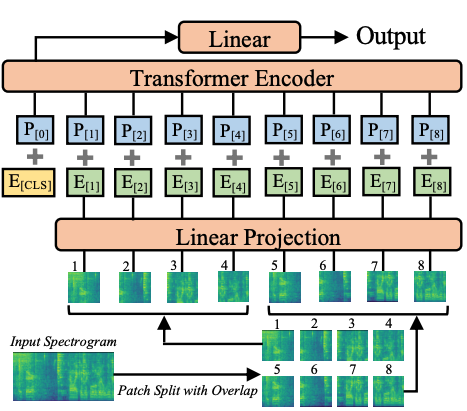
\includegraphics[trim=0 0 0 132, clip, scale=0.7]{figures/patchembedding.png}
    %\textcolor{red}{Insert Patch Embedding visualization.}
    \caption{The creation of a patch embedding from an input spectrogram.}
    \label{PatchEmbeddingFigure}
\end{figure}

\subsection{Architecture Modifications}

Originally, the Vision Transformer has been used on classification tasks where the output is not a sequence. \gls{ADT} is a sequence labeling task, and requires that the output is a sequence, where the time dimension matches the size of the input.

This can be solved by treating a group of patches from the patch embedding together as a timeframe, as long as we ensure that there the number of timeframes are a factor of the number of patches. Then the output of the Vision Transformer could be construed to match our intended output sequence.

\subsection{Implementation}

Initally, we transform the input spectrogram into a ($T \times D_e$) patch embedding. The Convolutional layer splits the spectrogram into ($T \times D_e / P \times P$) different patches. Added to these are a ($D_e / P \times P$) learnable positional embedding, providing positional information to each patch. These are then permuted and flattened, transforming them into our final patch embedding.

Afterwards, we combine it with a sinusoidal positional encoding, and successively apply $L$ attention blocks with number of heads $H$, identical in structure with those used in the Convolutional Transformer. Lastly, the linear layer outputs onset probabilities.

\begin{figure}[H]
    \hspace*{-0.5cm}
    \centering
    \begin{tikzpicture}[
    very thick,
    arrow/.style={
        -latex,
        very thick,
        rounded corners=0.2cm
    },
    do path picture/.style={%
        path picture={%
          \pgfpointdiff{\pgfpointanchor{path picture bounding box}{south west}}%
            {\pgfpointanchor{path picture bounding box}{north east}}%
          \pgfgetlastxy\x\y%
          \tikzset{x=\x/2,y=\y/2}%
          #1
        }
    },
    sin wave/.style={do path picture={    
        \draw [line cap=round] (-3/4,0)
        sin (-3/8,1/2) cos (0,0) sin (3/8,-1/2) cos (3/4,0);
        }
    }
    ]

\node[anchor=south, label=above:{Input Spectrogram}] at (1.25, -0.5){\footnotesize{($T \times D_\text{STFT}$)}};

\draw[arrow] (1.25, -0.5) -- (1.25, -1.5) node [rectangle,
rounded corners,
draw,
anchor=north,
fill=magenta!20,
minimum height=1cm,
minimum width=4cm
] (a) {Convolution: $D_e/P$ $(1 \times P)$};

\node [rectangle,
rounded corners,
draw,
anchor=north,
fill=yellow!20,
minimum height=1cm,
minimum width=4cm,
left = 1em of a,
] (b) {Positional Embedding};

\node[circle, 
draw, 
anchor=north,
minimum size=1em, 
inner sep=0pt
] at (-1.5, -2.75) (c) {$\mathbf{+}$};

\draw[arrow] (b) |- (c.west);
\draw[arrow] (a) |- (c.east);

\draw [arrow] (c) -- (-1.5, -3.6) node [rectangle,
rounded corners,
draw,
anchor=north,
fill=yellow!20,
minimum height=1cm,
minimum width=4cm,
] (d) {Flatten: $(T \times D_e)$};

\node [anchor=north,
above = 3em of c,
] (e) {Patch Embedding};

\begin{scope}[on background layer]
    \node[rectangle,
    fill=gray!10,
    rounded corners=5mm,
    draw,
    very thick,
    fit= (a) (b) (d) (e)] {};
\end{scope}

\node[circle, 
draw, 
anchor=north,
minimum size=1em, 
inner sep=0pt
] at (0, -6) (h) {$\mathbf{+}$};

\draw[arrow] (d) |- (h);

\node [circle, 
draw, 
sin wave, 
minimum size=2em, 
right=1em of h,
label={[align=left]east:Positional\\Encoding}
] (pe) {};

\draw (pe) -- (h);

\draw[arrow] (h) -- (0, -8) node[rectangle,
rounded corners,
draw,
anchor=north,
minimum size=1em,
inner sep=0pt,
fill=red!20,
minimum height=1cm,
minimum width=4cm,
label={west:$L\times$}
] (v) {Attention Block};

\draw[arrow] (v) -- (0, -9.5) node[rectangle, 
rounded corners, 
draw, 
anchor=north, 
fill=blue!20,
minimum height=1cm,
minimum width=4cm
] (w) {Linear (Sigmoid): $5$};

\draw[arrow] (w) -- (0, -11.0);

\node[anchor=north, label=below:{Output Probabilities}] at (0, -11.0){\footnotesize{($T \times 5$)}};


% ---- Attention Block ----
\draw (7.5, -4.5) node[rectangle,
rounded corners,
draw,
anchor=north,
fill=yellow!20,
label=north:Attention Block,
minimum height=0.75cm,
minimum width=4cm
] (i) {Layer normalization};

\draw[arrow] (i) -- (7.5, -6) node [rectangle,
rounded corners,
draw,
anchor=north,
fill=orange!20,
minimum height=1cm,
minimum width=4cm
] (j) {Multi-Head Attention: $H$};

\draw[arrow] (j.north)++(0, 0.4) -| ($(j.north) + (1.2,0)$);
\draw[arrow] (j.north)++(0, 0.4) -| ($(j.north) + (-1.2,0)$);

\draw (j) -- (7.5, -7.25) node[rectangle,
rounded corners,
draw,
anchor=north,
fill=yellow!20,
minimum height=0.75cm,
minimum width=4cm
] (k) {Dropout: $p = 0.1$};

\draw (k) -- (7.5, -8.125) node[rectangle,
rounded corners,
draw,
anchor=north,
fill=yellow!20,
minimum height=0.75cm,
minimum width=4cm
] (l) {Add \& Norm};

\coordinate (larrow) at ($(l.east) + (0.75, 0)$);
\draw[arrow] (j.north)++(0, 0.525) -| (larrow) |- (l.east);

\node[rectangle,
rounded corners,
draw,
anchor=north,
fill=cyan!20,
minimum height=0.75cm,
minimum width=4cm
] at (7.5, -10) (m) {Linear (GELU): $4 \times D_e$};

\coordinate (m1) at ($(m.north) + (0, 0.5)$);
\draw[arrow] (l) -- ($(m1.north) + (0, 0.1)$);

\draw (m) -- (7.5, -11) node[rectangle,
rounded corners,
draw,
anchor=north,
fill=cyan!20,
minimum height=0.75cm,
minimum width=4cm
] (n) {Linear: $D_e$};

\draw (n) -- (7.5, -12.25) node[rectangle,
rounded corners,
draw,
anchor=north,
fill=yellow!20,
minimum height=0.75cm,
minimum width=4cm
] (o) {Dropout: $p = 0.1$};

\draw (o) -- (7.5, -13.25) node[rectangle,
rounded corners,
draw,
anchor=north,
fill=yellow!20,
minimum height=0.75cm,
minimum width=4cm
] (p) {Add};

\draw[arrow] (m.north)++(0, 0.925) -| ($(p.east) + (0.75, 0)$) |- (p.east);

\coordinate (i1) at ($(i.north) + (0, 0.5)$);

\begin{scope}[on background layer]

    \node[rectangle,
    fill=gray!20,
    rounded corners=3mm,
    label={[name=mnlabel, yshift=-0.625cm]north:Feedforward},
    draw,
    very thick,
    fit=(m) (m1) (n)] (mn) {};
    \node[rectangle,
    fill=gray!10,
    rounded corners=5mm,
    draw,
    very thick,
    fit= (i1) (mn) (p) (larrow)] (imnp) {};
    \node[rectangle,
    fill=gray!20,
    rounded corners=3mm,
    label={[name=mnlabel, yshift=-0.625cm]north:Feedforward},
    draw,
    very thick,
    fit=(m) (m1) (n)] (mn) {};

    \begin{scope}[even odd rule]
        \path[clip] 
        (current bounding box.south west) rectangle (current bounding box.north east)
        ($(pe.north east) + (0, 0.25)$) rectangle ($(pe.south east) + (2.2, -0.25)$);
        \draw[thick, color=black!50] (v.north east) -- (imnp.north west);
        \draw[thick, color=black!50] (v.south east) -- (imnp.south west);
      \end{scope}
\end{scope};

\draw[arrow] (7.5, -3.25) node[anchor=south] {\footnotesize{($T \times D_e$)}} -- (i |- imnp.north);
\draw[arrow] (p |- imnp.south) -- (7.5, -14.75) node[anchor=north] {\footnotesize{($T \times D_e$)}};

\end{tikzpicture}
    \caption{Vision Transformer architecture structure.}
    \label{ViTFigure}
\end{figure}

\begin{table}[H]
    \centering
    \begin{tabular}{lr|c}
        \multicolumn{2}{c|}{Hyperparameter} & Values       \\
        \hline
        $P$ & Patch height      & \{7, 14, 21\} \\
        $H$ & Number of heads     & \{2, 4, 6, 8\} \\
        $L$ & Number of layers      & \{2, 4, 6, 8, 10\} \\
        $D_e$ & Embedding dimension      & \{72, 144, 288, 576\} \\
    \end{tabular}
    \caption{The different hyperparameters tuned to train the Vision Transformer.}
    \label{ViTHyperparams}
\end{table}

\chapter{Datasets}

\section{ENST+MDB}

The ENST-Drums dataset by Gillet and Richard~\cite{gillet_2006_7432188} has been one of the most commonly used \gls{ADT} datasets~\cite{8350302}. It features thorougly annotated drum samples by three drummers over different musical genres. Most of the tracks contain drum-only recordings, except the \textit{minus-one} subset, which is played together with a music accompaniement. As this thesis attends to \gls{DTM} tasks, we isolate our focus to this subset of tracks.

As this dataset contains separate audio files for performance and accompaniement, we additively combine them to create a singular respective mixture track. There exist many recordings from differently placed microphones of a single performance, however in this thesis, we solely selected the \textit{"wet mix"} due to it being a combined recording of all other microphone recordings, and its \textit{mix} showing resembelance of a polished performance track.

ENST-Drums contains 1.02 hours of music over 64 tracks.

Another well-known MedleyDB Drums dataset, from Southall et al.~\cite{southall2017mdb}. This dataset is built on top of Bittner et al.'s MedleyDB (MDB) dataset~\cite{bittner2014medleydb}, but re-annotated and specialized for \gls{ADT} related tasks. This dataset is, similar to ENST-Drums, also split into different stem tracks, such as isolated drum recordings and accompaniement. However, they also contain already-mixed \textit{full mix} tracks, which are the ones we use in this thesis.

MDB-Drums contains 0.35 hours of music over 23 tracks.

Both of these datasets distributes their audio in waveform files, and their annotations in text files. Annotations are formatted by onset time and instrument label. They are also relatively small, and contain thorough, real, annotated data. Due to these similarities, in this thesis they are combined together into a slightly larger ENST+MDB dataset.

In total, this dataset contains 1.37 hours of music over 87 tracks.

\subsection{Splits}

These two datasets do not have predefined train/validation/test splits, such that we decided to construct our own splits. From ENST-Drums, \textit{drummer1} and \textit{drummer2} make our training split. The remaining drummer, \textit{drummer3} is split in half, each for validation and test respectively. From MDB-Drums we do not have different explicit drummers, but instead split on specific genres. The explicit splits are given below, in table 4.1.

\textcolor{red}{Explain how this dataset gets train/val/test split. Give explicit titles for split as well. Here we've only given a text/explained split, however not the actual information. Probably do this in an appenix!}

\textcolor{red}{\textbf{ALSO VERIFY THAT SPLITS ARE AS WRITTEN. JUST TO BE SURE!}}


\begin{table}[H]
    \centering
    \begin{tabular}{l|lr}
        Split & ENST-Drums & MDB-Drums \\
        \hline
        Train & \textbf{"107\_minus-one\_salsa\_sticks"}      & \textbf{"MusicDelta\_Punk"} \\
        Validation & Number of heads     & \{2, 4, 6, 8\} \\
        Test & Number of layers      & \{2, 4, 6, 8, 10\} \\
    \end{tabular}
    \caption{The different tracks used for each respective train/validation/test split for this thesis.}
    \label{ENST+MDBSplits}
\end{table}

\subsection{Mapping}

\textcolor{red}{Maybe (or maybe not) explain the mapping from this to 5-instrument mapping. Also put this under a Appendix.}

\section{E-GMD}

The Expanded Groove MIDI Dataset (E-GMD) from Callender et al.~\cite{callender2020improvingperceptualqualitydrum} is a large \gls{ADT} dataset consisting of audio recordings from human drum performances annotated in MIDI. It is an expansion of Gillick et al.'s Groove MIDI Dataset (GMD)~\cite{pmlr-v97-gillick19a}.

GMD was created through recording human performances in MIDI format through a Roland TD-11 electronic drumkit. This dataset does not contain audio recordings, only MIDI files, such that it is not applicable for \gls{ADT}. To expand this dataset to be used with \gls{ADT}, Callender et al. re-recorded the MIDI sequences on a Roland TD-17 electronic drumkit in real-time on a \gls{DAW}. These re-recordings were done over a large amount of differing soundfonts (confusingly also called \textit{drumkits} on electronic drumkits), synthesizing several differently sounding audio recordings from a single MIDI performance~\cite{pmlr-v97-gillick19a, callender2020improvingperceptualqualitydrum}.

In contrast to the other dataset's utilized in this thesis, this dataset is not created for a \gls{DTM} task, but rather a \gls{DTD} task. This is due to all recordings containing solo, drum-only performances. In addition, as this data is recorded from human performances in a semi-manual nature, there exist some errors from the recording process \textit{"that resulted in unusable tracks."}~\cite{callender2020improvingperceptualqualitydrum}. The magnitude of these errors are not stated, however other authors propose that it might be as high as 20.5\% of the tracks with varying amounts of discrepancies~\cite{holz2021automatic}.

This dataset contains 444.5 hours of audio recordings, from 1,059 unique drum performances resampled to 45,537 MIDI sequences.

\subsection{Mapping}

\textcolor{red}{Maybe (or maybe not) explain the mapping from this to 5-instrument mapping. Also put this under a Appendix.}

\section{Slakh}

The Synthesized Lakh 2100 (Slakh) Dataset from Manilow et al.~\cite{8937170} is a synthesized version of a subset of the Lakh Dataset from Raffel~\cite{raffel2016learning}, that subset being a 2100 randomly selected tracks from Lakh where the MIDI files contain at least a piano, bass, guitar, and drums. These MIDI files are rendered and mixed into combined audio files, stored together with their respective original MIDI performances.

As mentioned, this dataset contains more instruments than just the drumset, such that it is originally meant for a \gls{AMT} task. However, due to each track being guaranteed to contain a drum performance, converting it to an \gls{ADT} task is trivial, and is done by selectively only utilizing the MIDI files corresponding to the drumset as our labels.

The original Slakh dataset was found to have data leakage between the different splits, and it is therefore recommended for transcription tasks to use a smaller subset, Slakh2100-redux, where this issue has been solved. Therefore, this is the dataset used for this thesis.
\textcolor{red}{Needs citation, other than the github and zenodo? \\ \url{https://github.com/ethman/slakh-utils}, \url{https://zenodo.org/records/4599666}}

This dataset contains 115 hours of audio recordings over 1709 different songs.

\subsection{Mapping}

\textcolor{red}{Maybe (or maybe not) explain the mapping from this to 5-instrument mapping. Also put this under a Appendix.}

\section{ADTOF-YT}

The Automatic Drums Transcription On Fire YouTube (ADTOF-YT) dataset from Zehren et al.~\cite{signals4040042} is a large \gls{ADT} dataset containing crowdsourced data, hence the YouTube suffix. Due to the crowdsourced nature of this dataset, it is possible to utilize large amounts of non-synthetic, human data, but with the tradeoff in which we can not guarantee its quality.

Contrary to the other datasets, this one is distributed in prepackaged TensorFlow datasets for each split, with datapoints as pairs of logarithmically filtered log-spectograms and sequence of instrument onset probabilities. This dataset also comes with a vocabulary of 5, and is thus the least diverse dataset in this thesis.

\textbf{Note that their sourcecode and dataset distributor informs us that the dataset contain mel-scale spectrograms, and not logarithmically filtered ones as we previousy proposed. However, through thorough code investigation and approximate reconstruction of original waveforms we hypothesize and conclude that this is a mistake.}
\textcolor{red}{Is this enough justification? Should I provide more information? If so, what exactly?}

The dataset contains 245 hours of music over 2924 tracks.

\subsection{Mapping}

Due to this dataset being distributed in a preprocessed nature, no re-mapping has been done, and the dataset is used "as is".

\section{SADTP}

The SADTP (Small Automatic Drum Transcription Performance) dataset is a novel dataset introduced in this thesis. It is a small dataset comprised of 16 songs with corresponding MIDI transcriptions. 

The \textit{performance} name alludes to the transcription being recorded live while listening to the songs on playback, with only minor post-processing. The transcriptions were recorded on a Roland TD-11 electric drumset, recording the MIDI perfomance to Apple's Garageband \gls{DAW}, and extracting them to separate MIDI files. This comes with a similarly to E-GMD, as this dataset also was recorded in a semi-manual nature, which opens the possibility for slight, human induced errors. The magnitude of such errors are however not known, but we speculate that it is small but not insignificant.

This dataset stands out, as it is the only one in this thesis not used for training. Its sole purpose is for zero-shot evaluation, and to provide information on the generalization ability for models trained on data from other sources.

The dataset contains 1.08 hours of music, which can be split into 977 non-overlapping 4 second datapoints (includes zero padding certain pieces for even partitioning).

\subsection{Mapping}

\textcolor{red}{Maybe (or maybe not) explain the mapping from this to 5-instrument mapping. Also put this under a Appendix.}

\section{Differences}

\textcolor{red}{Provide a table with information neatly gathered in a table. Such information should be size (total duration), vocabulary, real or synthetic data (human/non human), number of tracks. Should be like e.g. \cite{signals4040042,callender2020improvingperceptualqualitydrum} or others.}

\chapter{Methodology}\label{Methodology}

Though we perform 2 different studies, with 2 different intentions, the dataset preparation and model selection pipeline remains the same. 

\section{Data Preparation}

As mentioned, the different datasets are distributed in differening formats. A few transformations are done to unify them all as PyTorch datasets.

Due to the preprocessed nature of the ADTOF-YT dataset, the unification is trivial and simply denotes a transformation from a stored TensorFlow dataset to a PyTorch dataset. Otherwise it is kept "as is".

\subsection{Audio Files}

The others are however distributed in the Waveform Audio File Format (with the suffix \textit{.wav}) or using the Free Lossless Audio Codec (with the suffix \textit{.flac}). Both of these formats are loaded using the PyTorch library \texttt{Torchaudio} and converted to monophonic format through meaning over each side's waveform. If any datasets contain distinct drum and accompaniement audio (like e.g. ENST-Drums), these are additively mixed together.

After each track is loaded into a waveform, a zero-padding is added to the end of each sequence allowing for even partitioning into 4 second partitions. Then we turn the track into a spectrogram with 2048 fft's, and a window length of 2048. By keeping the hop length equal to the sampling rate divided by 100, the resulting spectrogram's timesteps represent a 10ms window of the original waveform.

After this, a filterbank is computed by generating 12 normalized logarithmically spaced filters, centered at 440Hz, and bounded over the interval [20Hz, 20,000Hz]. Applying this filterbank as a simple matrix multiplication over the spectrogram results in a logarithmically filtered spectrogram with $D_\text{STFT} = 84$ number of frequency bins. Lastly, we turn it into a log-spectrogram by applying a $\log_{10}$ operation to each cell, following an addition of 1 (preventing $\lim_{x \to 0}\log_{10}(x) = -\infty$ situations).

\subsection{Annotations}

The annotations are either distributed in specific formats as text files (with the suffix \textit{.txt}), or in MIDI files (with the suffix \textit{.mid} or \textit{.midi}), each one having a different transformation into a sequence of instrument onset probabilities.

The datasets declaring onsets in text files (ENST-Drums and MDB-Drums) follow a similar format, storing onsets on separate lines, each one containing the time in seconds for the onset, and its respective instrument ID, separated by a space or tab respectively. To convert this into the onset probability sequence, we convert the time into a timeframe index by turning the time into milliseconds, dividing by 10 to group into 10ms intervals, and rounding to the nearest integer. After this, we map the instrument ID into its respective class, and set that specific (timeframe, class) cell value to 1.

The data given in MIDI format, the annotations are parsed using the library \texttt{Partitura}, and loads the information into an array of MIDI events called \textit{notes}. These \textit{notes} contain information for each event, importantly time, pitch, and velocity. These events are very thorough, but strict instrument onsets can be isolated by restricting our view to notes with a non-zero velocity. Instruments are denoted by the event's pitch, and a mapping is done from each pitch to a respective class. The time is converted identically to the loading of the text annotations, turning them into timeframe indices. At last, we also here set each specific registered onset (timeframe, class) cell to 1.

In addition to this, we apply a \textit{target widening} step, setting values in timeframes adjacent to an instrument onset with a lower weight, equal to 0.5. These additional neighbouring \textit{soft labels} have shown to be benifical in countering sparsity in our labels following multiple works on beat transcription~\cite{9747048, signals4040042}.

\subsection{Splitting and Storing}

These spectrogram/onset sequence pairs are stored together in PyTorch's TensorDatasets, separated into each track's respective train/validation/test split, and stored into PyTorch pickle files (with the suffix \textit{.pt}). By doing all this preprocessing in advance, minimal preprocessing has to be done during runtime, increasing the efficiency of training.

\section{Preprocessing}

Most of the preprocessing is done during the data preparation step, however there are some remaining. Most importantly, a given model computes the mean and standard deviation of its training dataset, and uses these parameters to standardize its input data before prediction during runtime. 

Data normalization like this has been shown to increase the speed and stability of convergence during training and, in summary, producing models which better generalize to unseen data. Although the specific benefits depend on the normalization technique used, the general consensus is that normalization in itself is beneficial in machine learning, hence their ubiquitous use in state-of-the-art models~\cite{10056354}.

Another preprocessing step motivated by \gls{ADT} specific methods is the use of infrequency weights, which framewise weighs the loss based on the instrument onsets that are present at each frame. These weights are precomputed from the training dataset, and are, for each instrument, computed by what Cartwright and Bello call \textit{"the inverse estimated entropy of their event activity distribution"}~\cite{cartwright2018increasing}. Although they apply this to account for sparsity in data along different tasks, Zehren et al.~\cite{signals4040042} applied it to give more weight to infrequent instruments. 

These weights are computed by calculating the probability of an instrument $i$ appearing $p_i = \frac{n_i}{T}$ as the total number of onsets $n_\text{i}$ divided by the total number of timesteps $T$. With this probability we compute its inverse entropy, giving us our final weights $w_i = (-p_i\log{p_i} - (1 - p_i)\log{1 - p_i})^{-1}$. Note that our probability computation differs from the work of Cartwright and Bello, as we do not divide by the number of instruments~\cite{cartwright2018increasing}. 

\textcolor{red}{Should I mention anything on how the entropy is symmetric over 0.5? Such that a probability over 0.5 would lower our weights again, but how that is not a problem in ADT due to instrument onset inherently being sparse?}

\section{Training}

As mentioned, the \gls{ADT} task could be thought of as a sequence labeling task, where we each timeframe could have several instrument onsets present, taking the form of a 0 if an instrument is not present, and a 1 if it is. A natural loss function for this, where each value is handled as a separate independent probability distribution is the binary cross-entropy loss. Due to the numerical instability which can appear by applying a sigmoid activation function to our logits before computing the loss, we instead output our logits directly and utilize PyTorch's \texttt{BCEWithLogitsLoss} loss function, as recommended in their documentation \textcolor{red}{Do I need to cite this?}. It increases the numerical stability by taking advantage of the log-sum-exp trick, increasing numerical precision by avoiding underflow or overflow problems followed by significantly small or large input values.

With the choice by what to use, Adam was considered. This is an optimizer so ubiquitously used within the field of deep learning that when questioned with what optimizer to generally use authors like Sebastian Ruder state that \textit{".., Adam might be the best overall choice}~\cite{ruder2017overviewgradientdescentoptimization}. However contrary to this, the Adam optimizer has been shown to contain some issues, like its coupling of the weight decay term inside its gradient-based updates. Due to this, the choice instead fell on AdamW, a modified Adam implementation decoupling weight decay in whole from the gradient-based updates, and displaying a better ability to generalize.~\cite{kingma2017adammethodstochasticoptimization, bock2018improvementconvergenceproofadamoptimizer, loshchilov2019decoupledweightdecayregularization}

It was observed during training that the magnitude of the loss values could vary greatly and often displayed a tendancy to explode. To counteract this observation, we clip the gradients with a maximum norm set to 2. This addition significantly lowered the observed chance of exploding gradients occuring. 

Another addition which is frequenct in other \gls{ADT} works is the use of a learning rate scheduler. A learning rate scheduler keeps track of recent validation loss values, and if the minimum loss achieved plateaus (meaning it stop decreasing) for a certain number of epochs, the learning rate gets reducing by a given factor. In this thesis we reduce the learning rate by a factor of 5 if we observe 5 epochs of plateauing, with no improvement to our minimal validation loss~\cite{chang2024yourmt3+, signals4040042}. We also keep track of the general count of epochs since validation loss last improvement and perform an early stop if we ever observe 15 epochs without improvement.

\section{Postprocessing}

As mentioned, the model outputs a sequence of activation values, a 2 dimensional matrix with values on the interval $(0, 1)$ interpreted as the model's confidence in an instrument onset being present per frame. This can be utilized directly when computing our loss during training, however it is a difficult format to work with when talking about general performance, due to it rather representing a continuous confidence rather than discrete predictions. To suit this purpose, additional postprocessing is performed on the output.

First, we apply the aforementioned peak picking algorithm to isolate peaks in the model's onset confidence, intuitively being frames where the model is most confident in an instrument onset happening ~\cite{Bck2012EvaluatingTO, vogl2018multiinstrumentdrumtranscription}. Afterwards, we count a predicted onset if the given peak has a value larger or equal to 0.5. From this, it is trivial to compare predicted onsets with actual onsets, by greedily iterating our output sequence from the beginning, counting a prediction as a true positive if it happens within a 5 frame (50 ms) interval of a true onset, false positive if it happens outside such an interval, or false negative if a true onset happens with no prediction within said interval.

\begin{figure}[H]
    \centering
    %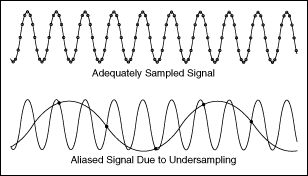
\includegraphics[scale=2.0]{figures/signalaliasing.png}
    \textcolor{red}{Could be useful showing transformation from output, to peak picked, to correct vs incorrect prediction.}
    %\caption{Example of aliasing in an undersampled signal.}
    %\label{AliasingFigure}
\end{figure}

These \gls{TP}, \gls{FP}, \gls{FN} predictions are then added together and used to compute the previously mentioned micro F1-score. For additional analysis, we also compute and store instrumentwise F1-scores.

\section{Model Selection}

For model training and selection we utilize the RayTune library~\cite{liaw2018tuneresearchplatformdistributed}. It simplifies the training of models by allowing us to input a training function, which metric to optimize for, hyperparameter spaces and search strategy, and additional configs. This simplifies our training, and through per-epoch reporting, it handles both checkpointing of model weights and best performing model selection for us.

Through RayTune, we train 15 different models (25 solely for the smallest dataset ENST+MDB), with hyperparameters tuned through bayesian optimization (see the next section~\ref{HyperparameterTuning}). Each model is also ran for at most 100 epochs. As mentioned, we perform an early stop if performance stops increasing. We utilize PyTorch's dataloaders for iterating the datasets, with a batch size of 128. And using the AdamW optimizer, as previously mentioned.

During each epoch of training, we evaluate the model on the training dataset's corresponding validation data. After training, the model with the highest Micro F1-score is selected. Due to the pre-split nature of most of our datasets, we utilize hold-out validation, with separate train, validation and test datasets. This is not only very common within \gls{ADT}~\cite{vogl2016recurrent, 8350302, chang2024yourmt3+}, but throughout the whole field of deep learning. Raschka mentions that \textit{"The holdout method is inarguably the simplest model evaluation technique"}~\cite{raschka2020modelevaluationmodelselection}, and might be one of the reasons for its popularity.
Then, we estimate its performance on unseen data through evaluating it on the test dataset. At last, said model is stored together with its corresponding weights, training config, and metrics.

\section{Hyperparameter Tuning}\label{HyperparameterTuning}

\subsection{Search Strategies}

There are several hyperparameters that are tuned for each model. One of the most thorough ways to tune these would be through a grid-search regime. Then, one would train and evaluate each possible hyperparameter combination, to find the best performing. However, this grows out of proportion fast, with an exponentially growing number of combinations based on the number of hyperparameters and their values, making it computationally expensive. Another way would be to use a random-search regime, where one randomly picks the combination of hyperparamters. This regime sacrifices hyperparameter combination coverage by increasing computational efficiency. The drawback with this approach however is its reliance on probability. During a given training trial, we might be unlucky with all our randomly selected hyperparameter combinations, leading to a suboptimal performing model.

A combination of these two regimes, almost utilizing "the best of both worlds" would be to use a bayesian optimization regime. It chooses its hyperparameter combinations in a random fashion, like random-search, but also uses previously trained models' performance values to "intelligently" perform later choices, focusing in on promising combinations. In this way, we reap the rewards of the random-search regime's computational efficiency, while keeping some of the thoroughness from the grid-search regime.

We utilize RayTune's implementation of \texttt{OptunaSearch}, a hyperparameter searching regime which uses Optuna, an automatic hyperparameter optimization software framework based on bayesian optimization~\cite{akiba2019optuna}. It has shown to be efficient in finding a good tradeoff between computation and performance, with authors like Shekhar et al. performing benchmarks on neural networks and showiung that \textit{"The performance score of Optuna is the highest for all datasets"}~\cite{shekhar2021comparative}.

\textcolor{red}{How much do I need to cite here?}

\subsection{Hyperparameters}

RayTune allows one to easily declare the search space for each of the hyperparameters. Every architecture-specific hyperparameter is chosen based on a random choice. In addition to this, we also tune the optimizer-specific learning rate and weight decay using a logarithmically uniform random sample. The specific spaces can be found below, in Table \ref{MethodHyperparams}.

\begin{table}[H]
    \centering
    \begin{tabular}{l|c}
        Hyperparameter & Search Space       \\
        \hline
        Learning Rate      & Log-uniform over $[1\cdot{10}^{-4}, 5\cdot{10}^{-3}]$ \\
        Weight Decay     & Log-uniform over $[1\cdot{10}^{-6}, 1\cdot{10}^{-2}]$ \\
        Architecture-specific Hyperparameters      & Random choice over each \\
    \end{tabular}
    \caption{The search space for each of the different hyperparameters. The architecture-specific hyperparameters can be found under each architecture in the Architecture chapter~\ref{Architectures}}
    \label{MethodHyperparams}
\end{table}

\chapter{Architecture Study}

This study's main purpose is to figure out how suited each architecture is for \gls{ADT}, more specifically \gls{DTM} tasks. This could help us figure out which architecture is superior for \gls{ADT}, if there are any similarities between architectures who perform similarly well, or if there are any architectures who perform poorly.

\section{Methodology}

We perform hyperparameter tuning and model selection to train a separate model for each architecture over each dataset. At last we test the model on each dataset's respective test split. As a result, we are left with performance measures on unseen data from the same distribution as those each model was train on. This will give us a good intuition into each architecture's ability to learn the task of \gls{ADT} and could help us estimate their generalization ability.

\section{Results}	

\begin{table}[H]
    \centering
    \hspace*{-0.6cm}
    \begin{tabular}{l|cccc}
        Architecture & ENST+MDB & E-GMD & Slakh & ADTOF-YT       \\
        \hline
        Recurrent Neural Network	& 0.6682 &	0.889 &	0.864 &	\textbf{0.9635} \\
        Convolutional Neural Network	& 0.7797 &	0.8744 &	0.8318 &	0.844 \\
        Convolutional Recurrent Neural Network	& \textbf{0.8132} &	\textbf{0.8935} &	\textbf{0.8959} &	0.9333 \\
        Convolutional Transformer	& 0.776 &	0.8831 &	0.8826 &	0.9535 \\
        Vision Transformer	& 0.5426 &	0.8779 &	0.879 &	\textbf{0.9635} \\
        
    \end{tabular}
    \caption{The Micro F1-score for each architecture, trained and tested on each dataset. The performances which are bolded represent the highest F1-score, and thus best performance, for that respective dataset.}
    \label{ArchitectureResultsTable}
\end{table}


\begin{figure}[H]
    \centering
    \hspace*{-0.8cm}
    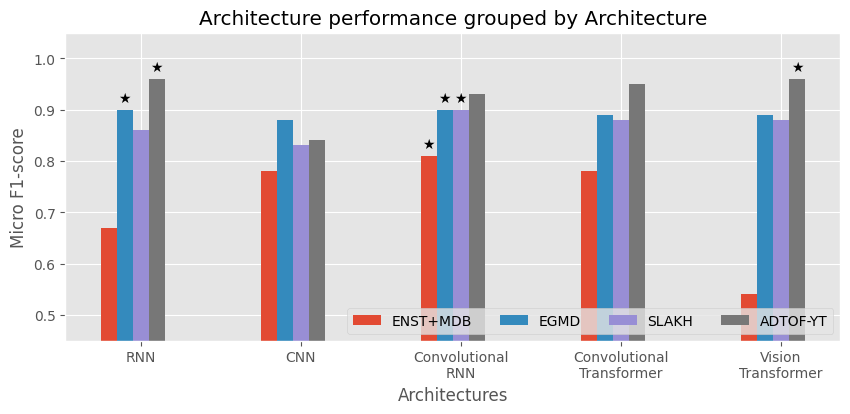
\includegraphics[scale=0.8]{figures/architectureperformancearchitecture.png}
    \caption{Comparison of Micro F1-scores for each dataset across the different architectures. Bars marked with a ($\star$) indicate the best performing architecture for each respective dataset.}
    \label{ArchitectureResultsArchitectureFigure}
\end{figure}

\begin{figure}[H]
    \centering
    \hspace*{-0.8cm}
    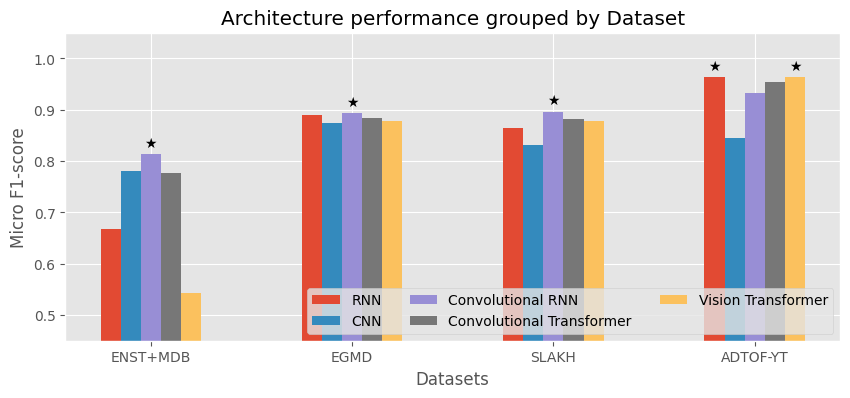
\includegraphics[scale=0.8]{figures/architectureperformancedataset.png}
    \caption{Comparison of Micro F1-scores for each architectures across the different dataset. Bars marked with a ($\star$) indicate the best performing architecture for each respective dataset.}
    \label{ArchitectureResultsDatasetFigure}
\end{figure}

\section{Discussion}

The architecture study's results are summarized in Table \ref{ArchitectureResultsTable} and visualized in Figures \ref{ArchitectureResultsArchitectureFigure} and \ref{ArchitectureResultsDatasetFigure}. From these results we can compare and discuss how each model performs, and speculate where the sources of their performances lie.

Firstly, it is evident that there does not seem to be one superior architecture when it comes to \gls{ADT}. There does not exist a single architecture outperforming the others across all the datasets, and the different architectures often share similarly high performances on most of the datasets. 

However, the convolutional recurrent neural network demonstrates the highest Micro F1-score on three of the four datasets (namely ENST+MDB, E-GMD and Slakh). It also provides a high, but not exceptional F1-score on the fourth (ADTOF-YT). The consistency of its high performance across the different properties of each dataset suggests that it is able to handle a wide variety of \gls{ADT} tasks, and that its performance may be high independent on the training dataset's size and complexity. In other words, it displays properties of being a architecture highly suitable for \gls{ADT} tasks. One could speculate that this suitability is provided by the strong inductive bias from the combination of convolutions and recurrent units, allowing for both initial spatial feature extraction as well as short-time temporal modelling.

The convolutional neural network displays a moderate performance across all datasets. It shows adequate performance on the smallest dataset (ENST+MDB), having the second highest F1-score. However, across all others (E-GMD, Slakh and ADTOF-YT) it displays the lowest. This relatively poor overall performance seems to indicate that the convolutional neural network currently is an inferior architecture for \gls{ADT} tasks, unless dataset size is limited, in which it could provide a viable architecture. It also shows the importance of explicitly leveraging the temporal dependencies within \gls{ADT}, as solely relying on the inductive bias of the convolutions didn't prove sufficient here.

This importance seems to be strengthened by the performance of the purely recurrent neural network, which has a surprisingly high performance across the datasets. In a way, it displays the opposite behaviour compared to the \gls{CNN}, displaying inadequate performance for the smallest dataset (ENST+MDB), but a relatively high performance for two of the others (E-GMD and Slakh), sharing the crown for the highest F1-score on the last (ADTOF-YT). The first dataset's low performance suggests that the inductive bias of the recurrent layers are "weaker" than the ones from convolutions, relying on a larger amount of data to accurately learn the task. Notably, it significantly outperforms the \gls{CRNN} on the last dataset, hinting that the inductive bias of the convolutions might "overpower" the model, proving so strong that it pulls the performance of the model down.



\chapter{Dataset Study}

This study's main purpose is to figure out how each dataset, and their characteristics, combined can influence a model's performance, both on- and \gls{OOD}. This could help us figure out how to utilize and combine current datasets, or how to intelligently construct future datasets, to optimize models' performance and generalization ability for \acrfull{ADT} and \acrfull{DTM}.

\section{Methodology}

We train convolutional recurrent neural networks, the best performing architecture from the first study, over several different combinations of the first four datasets ENST+MDB, E-GMD, Slakh, and ADTOF-YT. Datasets are combined as a union, where one epoch over the combined dataset would be equivalent to one epoch of both datasets separately. Each model is also evaluated on the remaining datasets, in addition to the SADPT dataset.

To get a comprehensive overview over how the different datasets could complement or contrast eachother's performances, without doing redundant experiments with diminishing returns, we select and train on a subset of all possible dataset combination. More specifically, we select 10 different combinations of datasets in such a way that we could extract valuable information about how their characteristics affect the resulting model's generalization ability.

\section{Results}

\begin{table}[H]
    \centering
    \hspace*{-1.0cm}
    \resizebox{1.13\linewidth}{!}{%
    \begin{tabular}{l|ccccc}
        Training Dataset & ENST+MDB & E-GMD & Slakh & ADTOF-YT & SADTP      \\
        \hline
        ENST+MDB	& 0.8132	& \cellcolor{blue!5} 0.5328	& \cellcolor{blue!5} 0.5294	& \cellcolor{blue!5} 0.5983	& \cellcolor{blue!5} 0.4165 \\
        E-GMD	& \cellcolor{blue!5} 0.4208	& \textbf{0.8935}	& \cellcolor{blue!5} 0.3532	& \cellcolor{blue!5} 0.3011	& \cellcolor{blue!5} 0.1833 \\
        SLAKH	& \cellcolor{blue!5} 0.7987	& \cellcolor{blue!5} 0.6676	& 0.8959	& \cellcolor{blue!5} 0.5922	& \cellcolor{blue!5} 0.4769 \\
        ADTOF-YT	& \cellcolor{blue!5} 0.8403	& \cellcolor{blue!5} 0.6253	& \cellcolor{blue!5} \underline{0.6546}	& 0.9333	& \cellcolor{blue!5} 0.607 \\
        \hline
        ENST+MDB + SLAKH	& 0.8394	& \cellcolor{blue!5} 0.6669	& 0.8983	& \cellcolor{blue!5} \underline{0.6324}	& \cellcolor{blue!5} 0.475 \\
        ENST+MDB + ADTOF-YT	& 0.863	& \cellcolor{blue!5} 0.6368	& \cellcolor{blue!5} 0.6342	& 0.9404	& \cellcolor{blue!5} \textbf{\underline{0.6189}} \\
        SLAKH + ADTOF-YT	& \cellcolor{blue!5} 0.8552	& \cellcolor{blue!5} 0.6493	& \textbf{0.9008}	& \textbf{0.965}	& \cellcolor{blue!5} 0.6178 \\
        \hline
        ENST+MDB + SLAKH + ADTOF-YT	& \textbf{0.8772}	& \cellcolor{blue!5} \underline{0.6768}	& 0.8942	& 0.9502	& \cellcolor{blue!5} 0.6122 \\
        E-GMD + SLAKH + ADTOF-YT	& \cellcolor{blue!5} \underline{0.8576}	& 0.8911	& 0.897	& 0.9401	& \cellcolor{blue!5} 0.6165 \\
        \hline
        ENST+MDB + E-GMD + SLAKH + ADTOF-YT	& 0.8646	& 0.8919	& 0.8932	& 0.9335	& \cellcolor{blue!5} 0.6169 \\
    \end{tabular}%
    }
    \caption{The Micro F1-score for a convolutional recurrent neural network trained over different combination of datasets, and tested on all datasets. The performances which are \textbf{bolded} represent the highest overall F1-score for the given dataset. Cells which are \colorbox{blue!10}{coloured light blue} represent \gls{OOD} evaluations. Values which are \underline{underlined} represent the highest possible F1-score of \gls{OOD} evaluations for the respective dataset.}
    \label{DatasetResultsTable}
\end{table}

\begin{table}[H]
    \centering
    \hspace*{-0.6cm}
    \begin{tabular}{l|cccc}
        Model & ENST+MDB & Slakh & ADTOF-YT      \\
        \hline
        SLAKH + ADTOF-YT & 0.8552	& \textbf{0.9008}	& \textbf{0.965} \\
        ENST+MDB + SLAKH + ADTOF-YT & \textbf{0.8772}	& 0.8942	& 0.9502 \\
        \hline
        ADTOF-RGW + ADTOF-YT~\cite{signals4040042} & 0.78/0.81* & - & 0.85 \\
        \hline
        MT3 (mixture)~\cite{gardner2022mt3multitaskmultitrackmusic} & - & 0.76 & - \\
        \hline
        YPTF.MoE+M~\cite{chang2024yourmt3+} & 0.8727**/- & 0.8456 & - \\
    \end{tabular}
    \caption{The Micro F1-score of selectively chosen convolutional recurrent neural networks from this dataset study, compared with best performing models from other literature over the three of the test sets. The performances which are \textbf{bolded} represent the highest overall F1-score for the given dataset for all compared models.
    (*) Zehren et. al tests on ENST-Drums and MDB-Drums separately and tests on different test splits than ours~\cite{signals4040042}.
    (**) Chang et. al only tests ENST-Drums and tests on a different test split than ours~\cite{chang2024yourmt3+}.}
    \label{DatasetComparisonTable}
\end{table}

\section{Discussion}

The results from the dataset study, summarized in Table \ref{DatasetResultsTable} highlight important insights regarding how dataset composition could affect and impact model generalization. These results clearly demonstrate that strategically combining \gls{ADT} datasets improve both on- and \acrfull{OOD} generalization.

Firstly, it is evident that each dataset exhibits great performance on test splits which distribution overlaps with their own training dataset, but a lesser performance when testing \gls{OOD}. There are several hypotheses one could propose for why this is the case, however one plausible one is that the datasets are characteristically varied enough in such a way that they each contrast eachother. This could give rise to this generalization penalty we see and explains the drop in performance. This generalization penalty also seem to be very uniform for different datasets, except one (E-GMD) which is talked about in the following paragraph. The best performing \gls{OOD} evaluations all lie in the Micro F1-score range of $0.6$ to $0.7$, except for the smallest dataset (ENST+MDB) which displays an F1-score of around $0.87$. Interestingly, the best performing \gls{OOD} evaluation for ENST+MDB is significantly close to its best performance overall. As we know, in contrast to the other datasets ENST+MDB consist of high quality, really precise \gls{DTM} data. A hypothesis is that this transcription quality of ENST+MDB more easily show the strength of the other model's, which might be hidden in the lesser quality of other test splits.

Another important observation, as mentioned, is that of E-GMD. As known, this dataset differs from the others by being a \acrfull{DTD} dataset, instead of a \gls{DTM} one. Despite its large size, it is the worst at generalizing to the others, and it is the worst performing model on all other datasets. However, it is worth to note that it also displays the best performance on itself. This helps reinforcing the differences between the tasks of \gls{DTD} and \gls{DTM}, showing how model's trained on differently tasked datasets are not directly applicable interchangeably. 

Building on this information we could inspect the opposite relationship. Notably, the other model's \gls{OOD} evaluation on E-GMD is comparable to that of their \gls{OOD} evaluations on themselves. This also helps strengthen the hypothesis that these tasks, \gls{DTD} and \gls{DTM}, display a complexity hierarchy where one seems to build upon the other. In other words, \gls{DTM} might be a more difficult transcription task than \gls{DTD}, but in return, a model trained for \gls{DTM} might be sufficient for \gls{DTD} tasks, and exhibits a zero-shot generalization ability which does not hold for the opposite.

One results that might merit discussion is the correlation between high ADTOF-YT performance and high SADTP performance. A high F1-score in the ADTOF-YT test split is accompanied by a relatively high \gls{OOD} F1-score for SADTP. Due to the crowdsourced nature of ADTOF-YT, and the SADTP consisting of contemporary and public music tracks, there might exist some overlap in their distribution which could explain this behaviour.\textcolor{red}{Maybe show correlation graph?}.

An insightful observation is that the best performance of all \gls{DTM} datasets from the architecture study, sees themselves beat by models trained on a combination of datasets. This is an important observation and shows that model performance often is enhanced by expanding the dataset size and variation. However, building upon what we discussed in the last paragraph, it is important to understand the differences between \gls{DTD} and \gls{DTM} datasets. As we observe, the best Micro F1-score for \gls{DTD} dataset comes from training data solely of \gls{DTD} data. The same holds the other way, in that the best performances on \gls{DTM} datasets happen when solely trained on \gls{DTM} data.

Secondly, take a look at the model trained on the largest amount of data, the combination of all datasets. This model exhibits superior performance across the board, however interestingly it does not achieve the highest Micro F1-score on any, though being very close. This strengthens the hypothesis that expanding the amount data will heighten generalization ability for a given model, and agrees with the current consensus that training dataset size is vital to achieving an optimally generalizing model~\cite{signals4040042, 9747048}. For future works it would be interesting to analyze how valuable data augmentation would be for \gls{ADT}, and if it affects generalization positively.

Lastly, in Table \ref{DatasetComparisonTable} we compare our best performing model's with other literature and giving remarkable insight. Note that not much literature exist with models evaluated on thsee datasets. Gardner et. al's MT3~\cite{gardner2022mt3multitaskmultitrackmusic} and Chang et. al's YPTF.MOE+M~\cite{chang2024yourmt3+} are general \gls{AMT} models, predicting several different instruments in addition to drums. They also present using the Offset F1-score terminology, equivalent to our Micro F1-score (also used by Zehren et. al~\cite{signals4040042}). Zehren et. al's ADTOF-RGW + ADTOF-YT is a \gls{DTM} model, similar to that of ours. Observably, we note that our model's outperform the others' by a singificant amount on both the Slakh and ADTOF-YT datasets. Due to the splits and datasets being a bit different for ENST+MDB, a direct comparison is a bit more difficult, but one could reason that our model's performance is comparable to that of YPTF.MOE+M~\cite{chang2024yourmt3+}. By comparing with results from other literature, we can put our model's performance into perspective and strengthens the argument that our combinations could in fact provide valuable advancements for the state-of-the-art in \gls{ADT} and \gls{DTM}.

In summary we can conclude that our results strongly indicate and strengthens our hypothesis that combining different datasets with variable characteristics, will help a model perform better on \gls{ADT} tasks, and could make them generalize better towards \acrfull{OOD} datasets. We also note that applicability of different \gls{ADT} tasks follow a relationship, where \gls{DTM} datasets generalize better on \gls{DTD} datasets than the inverse.

\textcolor{red}{I'm unsure if I've discussed enough (or too much of certain aspects) around the results presented in \ref{DatasetResultsTable}?}

% Include more chapters as required.
%%=========================================

% Print glossary containing Acronyms and Abbreviations
\printnoidxglossary[title=List of Acronyms and Abbreviations, type=\acronymtype]

% Include more appendices as required.
%%=========================================
\clearpage
\addcontentsline{toc}{chapter}{Bibliography}
\bibliographystyle{generators/myplainnat}
\bibliography{generators/refs}
\end{document}
